\subsection{线性不相交扩张}

在整个这一节中，\(\Omega\) 表示域 K 的一个扩张。

设 A 和 B 是 \(\Omega\) 的两个 K-子代数。存在一个代数同态 \(\varphi: \mathbf{A} \otimes_{\mathbf{K}} \mathbf{B} \to \Omega\) ，它把 \(x \otimes y\) 映到 \(xy\) 。\(\varphi\) 的像是 \(\Omega\) 中由 \(\mathbf{A} \cup \mathbf{B}\) 生成的子环 C。此外，根据 II，第 256 页，若 \((b_{\mu})\) 是 B 在 K 上的一组基，而 \((a_{\lambda})\) 是 A 在 K 上的一组基，则 C 与形如 \(\sum_{\mu} \alpha_{\mu} b_{\mu}\) （其中 \(\alpha_{\mu} \in \mathbf{A}\) ）的线性组合的集合一致，也是所有形如 \(\sum_{\lambda} \beta_{\lambda} a_{\lambda}\) （其中 \(\beta_{\lambda} \in \mathbf{B}\) ）的集合，以及所有形如 \(\sum_{\lambda, \mu} \gamma_{\lambda \mu} a_{\lambda} b_{\mu}\) （其中 \(\gamma_{\lambda \mu} \in \mathbf{K}\) ）的集合。

我们将称A和B在K上是线性不相交的，如果 \(\varphi\) 是 \(A \otimes_{K} B\) 到 C 上的同构。于是我们有 \(A \cap B = K\) ；B（相应地，A）的每个关于K的自由子集于是关于A（相应地，B）是自由的；反之，为使A和B在K上线性不相交，只需存在B在K上的一个基（例如）关于A是自由的（II，第256页及III，第469页）。

特别地，考虑 A 和 B 是 \(\Omega\) 的子扩张的情形。

命题5. --- 设E和F是包含在Ω中的K的两个扩张。

\begin{enumerate}
\def\labelenumi{\alph{enumi})}
\item
  如果 F 在 K 上具有有限次数，则 \(\Omega\) 中由 \(E \cup F\) 生成的子环是一个域，它与 \(\mathrm{E}(\mathrm{F})\) 一致，且 \(\mathrm{E}(\mathrm{F})\) 在 E 上的次数是有限的；我们有 \([\mathrm{E}(\mathrm{F}):\mathrm{E}] \leqslant [\mathrm{F}:\mathrm{K}]\) ，其中等号成立当且仅当 E 与 F 在 K 上线性不相交。在这种情况下 \(\mathrm{E}(\mathrm{F})\) 与 \(E \otimes_{K} F\) 是 E-同构的。
\item
  若E在K上具有有限次数，则 \(\mathrm{E}(\mathrm{F})=\mathrm{K}(\mathrm{E}\cup\mathrm{F})\) 在K上是有限次的。我们有 \([\mathrm{K}(\mathrm{E}\cup\mathrm{F}):\mathrm{K}]\leqslant[\mathrm{E}:\mathrm{K}][\mathrm{F}:\mathrm{K}]\) ，当且仅当E和F在K上线性不相交时等号成立。
\end{enumerate}

设 C 为 \(\Omega\) 中由 \(E \cup F\) 生成的子环；如果 \((b_j)_{1 \leq j \leq n}\) 是 \(F\) 在 \(K\) 上的一组基，则 \(C\) 是 \(\Omega\) 的由诸 \(b_j\) 生成的 E-向量子空间，因此 \(C\) 是一个有限秩代数，其秩 \(\leq n\) ，且位于 \(E\) 上；由于环 \(C\) 包含于一个域中，它是整环，因此由命题 1 的推论（V，第 10 页）可知它是一个域，从而 \(C = E(F)\) 且 \([E(F):E] \leq [F:K]\) 。关系式 \([E(F):E] = [F:K]\) 意味着诸 \(b_j\) 在 \(E\) 上线性无关，因此 \(E\) 与 \(F\) 在 \(K\) 上线性不相交；这证明了命题的第 \(a)\) 部分。第 \(b)\) 部分现在立即由 \([E(F):K] = [E(F):E][E:K]\) 这一事实得出。

设 E 和 F 是包含在 \(\Omega\) 中的 K 的扩张。若 E 和 F 在 K 上具有无限次数，则子环 \(C = K[E \cup F]\) 不一定是域 \(^{1}\) ；然而此时 C 的分式域恰好与 \(K(E \cup F)\) 一致。更一般地，设 A 是 E 的一个子环，使得 E 是 A 的分式域，并设 B 是 F 的一个子环，使得 F 是 B 的分式域；那么若 C 是 \(\Omega\) 中由 \(A \cup B\) 生成的子环，则 \(K(E \cup F)\) 与 C 的分式域一致，因为后一个域是 \(\Omega\) 中包含 C 的最小子域，且它包含 E 和 F。此外：

命题6. --- 设E和F是包含在Ω中的K的两个扩张，且A和B是Ω上K的两个子代数，使得E是A的分式域，F是B的分式域。则E和F在K上线性不相交当且仅当A和B在K上线性不相交。

该条件是显然必要的。反之，若A和B在K上线性不相交，则A和F也如此，因为若 \(\Omega\) 中的一族元素关于 B 是自由的，则它关于 B 的分式域 F 也是自由的（II，第 315 页，推论 1 及第 316 页，推论 3）；现在同样的论证表明 E 与 F 在 K 上是线性不相交的。

\(^{1}\) 只需考虑例如这样的情形：\(\Omega\) 是两个不定元 X 和 Y 上的有理分式域 \(\mathbf{K}(\mathbf{X},\mathbf{Y})\) ，且 \(\mathbf{E}=\mathbf{K}(\mathbf{X}),\mathbf{F}=\mathbf{K}(\mathbf{Y})\) 。

命题 7. --- 设 E 和 F 是包含在 Ω 中的 K 的两个扩张；若 E 和 F 在 K 上线性不相交，则 E 的每个子扩张和 F 的每个子扩张都在 K 上线性不相交。反之，若对于 E 和 F 的每一对有限生成子扩张 E'、F'（分别属于 E 和 F），E' 和 F' 都在 K 上线性不相交，则 E 和 F 在 K 上线性不相交。

因为 E 和 F 在 K 上线性不相交的条件可以这样表述：若 \((a_{\alpha})\) 是 E 中的一个自由族， \((b_{\beta})\) 是 F 中的一个自由族，则关系 \(\sum_{\alpha,\beta}\lambda_{\alpha\beta}a_{\alpha}b_{\beta}=0\) ，其中 \(\lambda_{\alpha\beta}\in K\) 蕴含 \(\lambda_{\alpha\beta}=0\) 对每一对下标成立。但若该条件对每一对有限自由族成立，则它对每一对自由族也成立。

因此，我们可以直观地说，线性不相交性是一个“有限特征”的性质。

命题 8. --- 设 E、F、G 是包含在 \(\Omega\) 中的域 K 的三个扩张，使得 \(F \subset G\) 。要使 E 和 G 在 K 上线性不相交，当且仅当 E 和 F 在 K 上线性不相交，且 E(F) 和 G 在 F 上线性不相交。

\pandocbounded{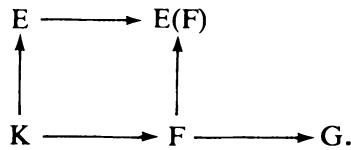
\includegraphics[keepaspectratio]{images/part001_e5f97af6.jpg}}\\
图 2.

条件必要性：假设 E 和 G 在 K 上线性不相交。那么 E 和 F 也如此（命题 7）；另一方面，若 B 是 E 在 K 上的一组基，则它也是代数 F{[}E{]} 在 F 上的一组基；由于由假设 B 在 G 上自由，F{[}E{]} 和 G 在 F 上线性不相交，且由命题 6，E(F) = F(E) 和 G 也如此。

条件充分性：用同样的记号，该条件蕴含 B 在 F 上自由，因此它是 F{[}E{]} 在 F 上的一组基；由于由假设 F{[}E{]} 和 G 在 F 上线性不相交，B 在 G 上自由，这表明 E 和 G 在 K 上线性不相交。

\section{代数扩张}

\subsection{代数的代数元素}

设 \(\mathbf{A}\) 是域 \(\mathbf{K}\) 上的一个代数，且 \(x\) 是 \(\mathbf{A}\) 的一个元素。有两种可能的情形：

\begin{enumerate}
\def\labelenumi{\alph{enumi})}
\item
  单项式族 \((x^{n})_{n\in\mathbb{N}}\) 在K上是自由的。这时我们称x在K上是超越的。存在多项式代数 K{[}X{]} 到 A 的由 x 生成的子代数 K{[}x{]} 上的一个同构，且后者在K上具有无限次数。
\item
  存在一个整数 \(n \geqslant 1\) ，使得这些单项式 \(1, x, \ldots, x^{n-1}, x^n\) 是线性相关的；这等同于说存在一个多项式 \(f \neq 0\) 属于 \(\mathbf{K}[\mathbf{X}]\) ，使得 \(f(x) = 0\) 。这时我们说 \(x\) 在 \(\mathbf{K}\) 上是代数的。满足上述性质的最小整数 \(n \geqslant 1\) 称为 \(x\) 在 \(\mathbf{K}\) 上的次数。如果 \(x\) 在 \(\mathbf{K}\) 上的次数是 \(n\) ，则单项式 \(1, x, \ldots, x^{n-1}\) 在 \(\mathbf{K}\) 上线性无关，并且存在元素 \(a_0, a_1, \ldots, a_{n-1}\) （属于 \(\mathbf{K}\)），使得
\end{enumerate}

\[
x ^ {n} = a _ {0} + a _ {1} x + \dots + a _ {n - 1} x ^ {n - 1}.
\]

多项式 \(f(\mathbf{X}) = \mathbf{X}^n - \sum_{k=0}^{n-1} a_k \mathbf{X}^k\) 是唯一的首一多项式，其次数为

\(n\) 的首一多项式，属于 \(\mathbf{K}[\mathbf{X}]\) ，使得 \(f(x) = 0\) ；它被称为 \(x\) 在 \(\mathbf{K}\) 上的极小多项式。

定理1. --- 设A是域K上的一个代数，x是A中在K上代数的元素，n是次数，f是x在K上的极小多项式。

\begin{enumerate}
\def\labelenumi{\alph{enumi})}
\item
  对于多项式 \(g \in \mathbf{K}[\mathbf{X}]\) ，要使它满足 \(g(x) = 0\) ，其充分必要条件是 \(g\) 是 \(f\) 的倍元。
\item
  映射 \(g \mapsto g(x)\) 通过过渡到商，定义了商代数 \(\mathbf{K}[\mathbf{X}] / (f)\) 到代数 \(\mathbf{K}[x]\) 上的一个同构，并且元素 1, x, \ldots, \(x^{n-1}\) 构成 \(\mathbf{K}[x]\) 在 \(\mathbf{K}\) 上的一组基。特别地， \([\mathbf{K}[x]: \mathbf{K}] = n\) 。
\item
  假设 A 是整环。则 K{[}x{]} 是域，且 f 是 K{[}X{]} 中唯一使得 \(f(x) = 0\) 的首一不可约多项式。
\item
  要使 \(x\) 在 \(\mathbf{A}\) 中可逆，其充分必要条件是 \(f(0) \neq 0\) ；于是我们有 \(x^{-1} \in \mathbf{K}[x]\) 。
\end{enumerate}

存在唯一的代数同态 \(\varphi: \mathbf{K}[\mathbf{X}] \to \mathbf{A}\) 使得 \(\varphi(\mathbf{X}) = x\) ；我们有 \(\varphi(\mathbf{P}) = \mathbf{P}(x)\) （对每个 \(\mathbf{P} \in \mathbf{K}[\mathbf{X}]\) ），并且 \(\varphi\) 的像等于 \(\mathbf{K}[x]\) 。设 \(\mathfrak{a}\) 是 \(\varphi\) 的核；根据构造，多项式 \(f\) （即 \(x\) 在 \(\mathbf{K}\) 上的极小多项式）属于 \(\mathfrak{a}\) ，并且它是 \(\mathfrak{a}\) 中次数最小的首一多项式。因此（IV，第～11页，命题11）我们有 \(\mathfrak{a} = (f)\) ，从而得到 \(a\) ）。断言 \(b\) ）立即由 \(a\) ）以及IV第～11页命题10的推论得出。

假设A是一个整环。则代数 K{[}x{]} 是一个整环且在K上具有有限次数，因此它是一个域（V，第～10页，推论）。于是 K{[}x{]} 的理想 (f) 是极大的，这意味着 f 在 K{[}X{]} 中不可约（IV，第～13页）。最后，设 g 是 K{[}X{]} 中一个使 \(g(x) = 0\) 的首一不可约多项式；由 a) 可知它是 f 的倍元，因此 g = f，这就证明了 c)。

还需证明 \(d\) ）。存在一个多项式 \(g \in \mathbf{K}[\mathbf{X}]\) ，其次数为 \(n - 1\) ，以及一个元素 \(a\) （属于 \(\mathbf{K}\)），使得 \(f(\mathbf{X}) = \mathbf{X}g(\mathbf{X}) + a\) ，从而 \(f(0) = a\) 。若 \(a = 0\) ，则我们有 \(xg(x) = f(x) = 0\) ，而 \(g(x) \neq 0\) ，于是 \(x\) 在 \(\mathbf{A}\) 中不可逆。另一方面，若 \(a \neq 0\) ，则我们有 \(x \cdot [-a^{-1}g(x)] = 1\) ，所以 \(x\) 在 \(\mathbf{A}\) 中可逆，且 \(x^{-1} = -a^{-1}g(x)\) 。

推论1. --- 设A是域K上的一个代数。对于A的元素x，它在K上是代数的当且仅当由x生成的A的子代数 \(K[x]\) 在K上为有限次。特别地，若A在K上为有限次，则A的每个元素都在K上代数。

推论2. —— 设E是K的一个扩域，A是E上的一个代数，x是A中在K上代数的元素。则x在E上是代数的，x在E上的极小多项式整除x在K上的极小多项式，且x在E上的次数至多等于x在K上的次数。

设 \(f\) 为 \(x\) 在 \(\mathbf{K}\) 上的极小多项式；我们有 \(f(x) = 0\) 且 \(f \in \operatorname{E}[\mathbf{X}]\) ，因此 \(x\) 在 \(\mathbf{E}\) 上是代数的，且 \(f\) 是 \(x\) 在 \(\mathbf{E}\) 上的极小多项式的倍式（定理1，a））。

注记. --- 设 E 是域 K 的一个扩域，且 x 是 E 中一个元素，它是某个首一不可约多项式 \(f \in K[X]\) 的根。则定理 1，c）表明 f 是 x 在 K 上的极小多项式。

例子。--- * 1) 在复数域 C 中，数 i 在素域 Q 上是次数为 2 的代数数；因为如果 \(f(\mathbf{X}) = \mathbf{X}^{2} + 1\) ，则 \(f(i) = 0\) ，且 \(x^{2} + 1 \neq 0\) 对所有 \(x \in Q\) 成立，因此 \(i \notin Q\) 。于是域 \(\mathbf{Q}(i)\) 是 Q 的 2 次扩张；它由所有形如 \(a + bi\) 的数组成，其中a、b是有理数。同样地，i在实数域R上是2次代数数，且C是R的2次扩张。

\begin{enumerate}
\def\labelenumi{\arabic{enumi})}
\setcounter{enumi}{1}
\tightlist
\item
  设K是一个域，F 是 K 上的一元有理函数域 \(\mathrm{K}(\mathrm{X})\) 。设E为 F 的子域 \(\mathrm{K}(\mathrm{X}^{3})\) ；我们有 \(\mathrm{F} = \mathrm{E}(\mathrm{X})\) 且X在E上是代数的，因为它是多项式 \(Y^{3} - X^{3}\) 的根，该多项式属于环 \(E[Y]\) ；该多项式在 \(E[Y]\) 中不可约，因为若不然，它至少会有一个一次因子，从而存在两个非零多项式 \(u(\mathrm{X})\) , \(v(\mathrm{X})\) （属于 \(K[X]\) ）使得 \((u(\mathrm{X}^{3}))^{3} = \mathrm{X}^{3}(v(\mathrm{X}^{3}))^{3}\) ，这是荒谬的，因为若 m 和 n 分别是 u 和 v 的次数，这将意味着 \(9m = 9n + 3\) ，或 \(3m = 3n + 1\) 。因此，域 F 在 E 上的次数为 3，且 F 中的每个元素都可以唯一地写成线性组合 \(f(\mathrm{X}^{3}) + \mathrm{X}g(\mathrm{X}^{3}) + \mathrm{X}^{2}h(\mathrm{X}^{3})\) ，其中 f、g、h 是三个属于 \(\mathrm{K}(\mathrm{X})\) 的有理分式。
\end{enumerate}

*3) 在实数域 \(\mathbf{R}\) 中，可以证明 \(^1\) 数 \(\pi\) 在素域 \(\mathbf{Q}\) 上是超越的。*

\subsection{代数扩张}

定义1. —— 域K的扩域E称为（在K上）代数的，如果E的每个元素都在K上是代数的。域K的扩域E若不是代数的，则称为（在K上）超越的。

命题1. --- 要使K的扩域E成为代数扩张，其充分必要条件是E的每一个子K-代数A都是一个域。

条件是必要的：如果 E 在 K 上是代数的，且 \(x \neq 0\) 是 E 的子 K-代数 A 的一个元素，则由 V，第 16 页，定理 1，d) 可知 \(x^{-1} \in K[x] \subset A\) 。因此 A 是一个域。

条件是充分的：如果它被满足且 x 是 E 中一个 \(\neq 0\) 的元素，则环 K{[}x{]} 是一个域，因此 \(x^{-1} \in K[x]\) ；换言之，存在一个多项式 \(g \in K[X]\) 使得 \(x^{-1} = g(x)\) ，或者也有 \(xg(x) - 1 = 0\) ；这表明 x 在 K 上是代数的，因此 E 是 K 的一个代数扩张。

命题2. --- 如果K的一个扩张E的次数为有限数n，则E是代数的，且E中每个元素在K上的次数整除n。

因为，给定 \(x \in \mathbb{E}\) , \([\mathbf{K}(x): \mathbf{K}]\) 是有限的且整除 \(n(\mathbf{V}, p. 10, \text{Cor. } 1)\) ，因此 \(x\) 在 \(\mathbf{K}(\mathbf{V}, p. 17, \text{Cor. } 1)\) 上是代数的。

* 存在无限次数的代数扩张，例如有限域的代数闭包（V，第24页，注记4）。*

定理2. --- 设E是K的有限生成扩张，由元素 \(a_1, \ldots, a_m\) 生成，这些元素是K上的代数元；则E是K的有限次扩张。若 \(a_i\) 在 K 上（相对于 \(a_1, a_2, \ldots, a_{i-1}\) ) 的次数是 \(n_i\) （对于 \(1 \leq i \leq m\) )，则 E 在 K 上的次数为 \(n_1 n_2 \ldots n_m\) 且元素 \(a_1^{\nu_1} a_2^{\nu_2} \ldots a_m^{\nu_m}\) ( \(0 \leq \nu_i \leq n_i - 1\) ) 构成 E 在 K 上的一组基。

元素 \(a_i^{\nu_i}\) ( \(0 \leqslant \nu_i \leqslant n_i - 1\) ) 构成 \(K(a_1, a_2, \ldots, a_i)\) 在 \(K(a_1, a_2, \ldots, a_{i-1})\) 上的一组基，这由 V 第 16 页定理 1 b) 可知；因此该定理通过对 \(m\) 归纳，由第二卷第 222 页命题 25 得出。

推论1. --- 设E是K的一个扩域，且A是E的一个由在K上代数的元素组成的子集。则K(A)在K上是代数的，并且我们有K{[}A{]} = K(A)。

因为每个 \(x \in \mathrm{K}(\mathrm{A})\) 都属于一个域 \(\mathrm{K}(\mathrm{F})\) ，其中 F 是 A 的有限子集（V，第 11 页，推论）；现在 \(\mathrm{K}(\mathrm{F})\) 在 K 上是代数的，且由定理2等于 \(\mathrm{K}[\mathrm{F}]\) ，因此x在K上是代数的，且 \(\mathrm{K}(\mathrm{A}) = \mathrm{K}[\mathrm{A}]\) 。

推论2. --- 设L是K的一个扩张，E、F是L的子扩张。若F在K上是代数的，则子环K{[}E, F{]} 由 E ∪ F 生成的 L 是一个域，它等于 E(F)，并且在 E 上是代数的。

F 的每个元素在 K 上是代数的，因此在 E 上也是代数的（V，第 17 页，推论 2），从而 \(E(F)\) 是 E 的一个代数扩张，并且我们有 \(E(F) = E[F]\) 由推论1可知。

注记。--- 1) 采用定理 2 的记号，E = K{[}a₁, a₂, \ldots, aₘ{]} 因此 E 同构于商 K{[}X₁, X₂, \ldots, Xₘ{]}/α；由于 E 是域，α 是 K{[}X₁, \ldots, Xₘ{]} 中的极大理想。

\begin{enumerate}
\def\labelenumi{\arabic{enumi})}
\setcounter{enumi}{1}
\tightlist
\item
  设 \(\mathbf{E}\) 是 \(\mathbf{K}\) 的代数扩张，且次数无限。由定理2，存在一个无限序列 \((a_n)_{n \geq 1}\) ，其元素属于 \(\mathbf{E}\) ，使得 \(a_n \notin \mathbf{K}(a_1, a_2, \ldots, a_{n-1})\) ；定理2进一步表明 \(\mathbf{K}(a_1, a_2, \ldots, a_n)\) 在 \(\mathbf{K}\) 上的次数取任意大的值。换句话说，如果E是K的代数扩张，且次数 \([F:K]\) （即 E 的在 K 上为有限次的子扩张 F 的次数）有界，则 E 是 K 的有限次扩张。
\end{enumerate}

\subsection{代数扩张的传递性。在扩域中相对代数闭的域}

命题3. --- 设E和F是域K的两个扩域，使得 \(K \subset E \subset F\) 。要使 F 在 K 上是代数的，当且仅当 E 在 K 上是代数的且 F 在 E 上是代数的。

该条件是必要的，由 V，第 17 页，推论 2 可知。下面证明其充分性。设 x 为 F 的任意元素；它在 E 上是代数的；设 \(g \in E[X]\) 为其在 E 上的极小多项式。若 A 为 g 的系数的（有限）集合，则 \(g \in K(A)[X]\) ，因此 x 在 \(K(A)\) 上是代数的，且 \(K(A \cup \{x\}) = K(A)(x)\) 在 \(K(A)\) 上是有限次的。现在 \(A \subset E\) 且E在K上是代数的，因此 \(K(A)\) 在K上是有限次的（由定理2）。因此（第V卷，第10页，定理1）， \(K(A \cup \{x\})\) 在K上是有限次的，这表明x在K上是代数的（V，第18页，命题2）。

定义2. —— 域E的子域K称为在E中相对代数闭的，如果E中每个在K上代数的元素都属于K。

这等价于说，K 是包含在 E 中的唯一的 K 的代数扩张。每个域K在自身中都是相对代数闭的。在第4节中，我们将研究在每个扩域中都是相对代数闭的域。

命题4. --- 设E是域K的一个扩域；E中在K上代数的元素之集L构成E的一个子扩域，且L在E中相对代数闭。

因为域 \(\mathbf{K}(\mathbf{L})\) 在 \(\mathbf{K}\) 上是代数的（定理2的推论1），因此 \(\mathbf{K}(\mathbf{L}) \subset \mathbf{L}\) ；由此可得 \(\mathbf{K}(\mathbf{L}) = \mathbf{L}\) ，且 \(\mathbf{L}\) 是一个域。另一方面，如果 \(x \in \mathbf{E}\) 在 \(\mathbf{L}\) 上是代数的，则它在 \(\mathbf{K}\) 上也是代数的（命题3），因此属于 \(\mathbf{L}\) 。

K在E中的相对代数闭包是指E中所有在K上代数的元素组成的K的扩张L；它是包含在E中的K的最大代数扩张。

\section{代数闭扩张}

\subsection{代数闭域}

命题1. --- 设K为一个域；则以下性质等价：

(AC) \(\mathbf{K}[\mathbf{X}]\) 中的每个非常数多项式在 \(\mathbf{K}[\mathbf{X}]\) 中分裂成若干个一次多项式（可以相同也可以不同）的乘积。

(AC') K{[}X{]} 的每一个非常数多项式在K中至少有一个根。

(AC'') K{[}X{]} 中的每一个不可约多项式的次数都为1。

(AC''') K 的每个代数扩张的次数均为 1（换言之，K 在 K 的每个扩域中都是相对代数闭的）。

我们首先证明性质 (AC)、(AC') 与 (AC'') 的等价性。显然 (AC) 蕴含 (AC'')。由于 K{[}X{]} 的每个非常数多项式可被一个不可约多项式整除（IV，第13页，命题13），且 K{[}X{]} 中每个次数为 1 的多项式显然在K中有一个根，我们看到(AC'')蕴含(AC')。条件(AC')通过对n的归纳，蕴含 K{[}X{]} 中每个n次多项式都是n个一次多项式的乘积（IV，第14页，命题1），因此(AC')蕴含(AC)。

还需证明 \((AC'')\) 与 \((AC''')\) 是等价的。若 \((AC'')\) 成立，则K的扩域L中每个在K上代数的元素次数都为1（V，第16页，定理1），因此属于K，这便确立了 \((AC''')\) 。反之，设 f 是一个次数为 \(n \geqslant 1\) 的不可约多项式，它属于 K{[}X{]}；商代数 \(K[X]/(f)\) 在 K 上的次数为 n 且是一个域，因此是 K 的一个 n 次代数扩张（V，第 18 页，命题 2）。现在显然 \((AC''')\) 蕴含 \((AC'')\) 。

定义 1. --- 一个域 K 被称为代数闭的，如果它满足（等价的）性质 (AC)、(AC')、(AC'')、(AC''')。

* 例 1. --- 复数域 \(\mathbf{C}\) 是代数闭域（Gen.～Top., VIII, p.～100）。*

一个域 K 在扩域 E 中相对代数闭，并不一定意味着 K 是代数闭的（事实上，每个域在自身中都是相对代数闭的，并且存在不是代数闭的域，例如 Q 或 \(F_{p}\) * 或 \(R_{*}\) ）。然而：

命题2。——设 \(\Omega\) 为一个代数闭域，K 为 \(\Omega\) 的一个子域。那么 K 的相对代数闭包 \(\bar{\mathbf{K}}\) （在 \(\Omega\) 中）是一个代数闭域。

设 \(f\) 为 \(\bar{\mathbf{K}}[\mathbf{X}] \subset \Omega[\mathbf{X}]\) 中的一个非常数多项式。由于 \(\Omega\) 是代数闭的，多项式 \(f\) 在 \(\Omega\) 中至少有一个根，且由于这个根在 \(\bar{\mathbf{K}}\) 上是代数的，它属于 \(\bar{\mathbf{K}}\) （V，第19页，命题4）。因此 \(\bar{\mathbf{K}}\) 满足 (AC')。

例2.——根据命题2，所有在Q上代数的复数（通常简称为代数数）构成一个代数闭域。

每个代数闭域都是无限的。

设 \(\mathbf{K}\) 为一个有限域，并令 \(f(\mathbf{X}) = 1 + \prod_{a\in \mathbf{K}}(\mathbf{X} - a)\) 。多项式

\(f \in K[X]\) 是非常数的，并且 \(f(a) = 1\) 对每个 \(a \in K\) 成立。因此，域K不满足(AC')，从而不是代数闭的。

定理1（施泰尼茨）。——设K为一个域，E为K的一个代数扩张，且 \(\Omega\) 为K的一个代数闭扩张；则存在一个 E 到 \(\Omega\) 的 K-同态。

由V，第13页，附注，存在一个扩域 \(\Omega'\) （\(\Omega\) 的扩张）以及一个K-同态 \(u\) ，它将 E 映入 \(\Omega'\) 。设 \(x \in E\) ；由于 \(x\) 在K上是代数的， \(u(x)\) 在 \(u(\mathbf{K})\) 上是代数的，并且更有理由在 \(\Omega\) 上是代数的（V，第17页，推论2）；由于 \(\Omega\) 是代数闭的，因此我们有 \(u(x) \in \Omega\) 。由此可知， \(u\) 将 E 映入 \(\Omega\) 。

\subsection{分裂扩张}

定义2. --- 设K为一个域，且 \((f_{i})_{i\in I}\) 为 K{[}X{]} 中非常数多项式的一个族。所谓 \((f_{i})_{i\in I}\) 的一个分裂扩张，我们指的是K的任意满足以下性质的扩张E：

\begin{enumerate}
\def\labelenumi{\alph{enumi})}
\item
  对于每个 \(i \in \mathbf{I}\) ，多项式 \(f_i\) 在 \(\mathbf{E}[\mathbf{X}]\) 中分裂成若干个一次多项式的乘积。
\item
  对于每个 \(i \in I\) ，令 \(\mathbf{R}_i\) 为多项式 \(f_i\) 在 \(E\) 中的根集，则 \(E = K\left(\bigcup_{i \in I} \mathbf{R}_i\right)\) 。
\end{enumerate}

有时使用“分裂域”一词代替“分裂扩张”。

注记。--- 1) 对于每个 \(i \in I\) ，令 \(c_i\) 是 K 的一个非零元素，并令 \(f_i' = c_i f_i\) 。那么显然，族 \((f_i)_{i \in I}\) 的每个分裂扩张也是族 \((f_i')_{i \in I}\) 的一个分裂扩张，反之亦然。特别地，在研究分裂扩张时，我们可以仅限于考虑首一多项式的情形。

\begin{enumerate}
\def\labelenumi{\arabic{enumi})}
\setcounter{enumi}{1}
\tightlist
\item
  假设I是有限的，并设 \(f = \prod_{i \in I} f_i\) 。利用多项式分解为不可约因子的唯一性
\end{enumerate}

（于 E{[}X{]} 中）（IV，第 13 页，命题 13），我们可以容易地证明，多项式 f 的一个分裂扩张是族 \((f_{i})_{i \in I}\) 的一个分裂扩张，反之亦然。换言之，有限族的情形可以归结为单个多项式的情形。

\begin{enumerate}
\def\labelenumi{\arabic{enumi})}
\setcounter{enumi}{2}
\tightlist
\item
  设 \(f \in K[X]\) 是一个次数为 \(\geqslant 1\) 的多项式，并设 E 是 f 的一个分裂扩张。若 \(x_{1}, \ldots, x_{n}\) 是 f 在 E 中的根，则我们有 \(\mathrm{E} = \mathrm{K}(x_{1}, \ldots, x_{n})\) ，且 \([E : K]\) 是有限的（V，第18页，定理2）；但E可能不同于由单个根生成的子域 \(\mathrm{K}(x_{1}), \ldots, \mathrm{K}(x_{n})\) ；即使f是不可约的，这种情况也可能发生 \(^{1}\) 。然而我们注意到，当f不可约时，这些域 \(\mathrm{K}(x_{i})\) 在 K 上的次数均为 n，并且当 E 等于其中之一时，我们有 \([E : K] = n\) ，因此 \(\mathrm{E} = \mathrm{K}(x_{1}) = \cdots = \mathrm{K}(x_{n})\) 。
\end{enumerate}

命题 4. --- 设 K 为一个域，且 \((f_{i})_{i\in I}\) 为 K{[}X{]} 中非常数多项式的一个族；那么存在族 \((f_{i})_{i\in I}\) 的一个分裂扩张。

我们可以取这些多项式 \(f_{i}\) 为首一的（注记1）。设 \(i \in I\) 并令 \(f_{i}\) 的次数为 \(d_{i}\) 。根据IV，第73页，命题5，存在一个交换代数 \(A_{i}\) （在 \(K\) 上），它不约化为 0，以及元素 \(\xi_{i,1}, \ldots, \xi_{i,d_{i}}\) （属于 \(A_{i}\)），使得：

\begin{enumerate}
\def\labelenumi{\alph{enumi})}
\item
  该代数 \(\mathbf{A}_i\) 由 \((\xi_{i,1},\dots,\xi_{i,d_i})\) 生成；
\item
  我们有 \(f_{i}(\mathbf{X}) = \prod_{k=1}^{d_{i}} (\mathbf{X} - \xi_{i,k})\) 在 \(\mathbf{A}_i[\mathbf{X}]\) 中成立。
\end{enumerate}

设 A 为代数族 \((\mathbf{A}_{i})_{i\in I}\) 的张量积，并且令 \(\varphi_{i}\) 为 \(A_{i}\) 到 A 中的典范同态（III，第 470 页）。此时代数 A 是交换的且不约化为 0；因此由 Krull 定理（I，第 104 页），在 A 中存在一个极大理想 a，并且 \(E = A/a\) 是域K的扩张。

用 \(\psi\) 表示 A 到 E 的典范同态，并令 \(x_{i,k} = \psi (\varphi_i(\xi_{i,k}))\) （对 \(i\in I\) 及 \(1\leqslant k\leqslant d_i\)）。由于代数 A 由 \(\cup \varphi_i(A_i)\) 生成，扩张 E 由族 \((x_{i,k})\) 生成。进一步地，对每个 \(i\in I\) 我们有

\(f_{i}(\mathbf{X}) = \prod_{k=1}^{d_{i}} (\mathbf{X} - x_{i,k})\) 在 E{[}X{]} 中成立。因此，E 是族 \((f_{i})_{i \in I}\) 的一个分裂扩张。

命题5. --- 设 K 是一个域， \((f_i)_{i \in I}\) 为 K{[}X{]} 中非常数多项式的一个族，E 是 K 的一个扩张，且 F、F' 是 E 的子扩张，它们各自是 \((f_i)_{i \in I}\) 的一个分裂扩张。则 F = F'。

设 \(\mathbf{R}_i\) 为多项式 \(f_i\) 在 \(\mathbf{E}\) 中的根集，且 \(\mathbf{R} = \bigcup_{i\in I}\mathbf{R}_i\) 。由于 \(f_i\) 是

F{[}X{]} 中若干一次多项式的乘积，我们有 \(R_{i} \subset F\) 。根据定义2，我们有 \(F = K(R)\) ；同样地，我们发现 \(F' = K(R)\) 。

推论。--- 设 K 是一个域， \((f_{i})_{i\in I}\) 为 K{[}X{]} 中非常数多项式的一个族，且 F, F' 是 \((f_{i})_{i\in I}\) 的分裂扩张。则存在一个从 F 到 F' 的 K-同构。

这由命题5以及V，第13页，命题4的推论得出。

\subsection{域的代数闭包}

定义3.——设K是一个域。所谓K的代数闭包，我们指的是K的任意一个既是代数的又是代数闭的扩张。

例子.—— * 1) 复数域C是实数域R的代数闭包（Gen.～Top., VIII, p.～100） *

\begin{enumerate}
\def\labelenumi{\arabic{enumi})}
\setcounter{enumi}{1}
\tightlist
\item
  设 K 为一个域，且 \(\Omega\) 为 K 的一个代数闭扩张。如果 \(\bar{K}\) 是 K 在 \(\Omega\) 中的相对代数闭包，则由V，第20页，命题2， \(\bar{K}\) 是 K 的一个代数闭包。* 特别地，全体代数数构成的域（V，第 20 页，习题 2）是有理数域 Q 的一个代数闭包。*
\end{enumerate}

命题6。——设 \(\Omega\) 是域 \(K\) 的一个扩张。要使 \(\Omega\) 是 \(K\) 的一个代数闭包，必要且充分的条件是：它应为代数的，并且 \(K[X]\) 中的每个非常数多项式应在 \(\Omega[X]\) 中分解为若干个一次因式的乘积。

该条件由 (AC) 知是必要的。反之，假设 \(\Omega\) 在K上是代数的，并且 K{[}X{]} 上的每一个非常数多项式在 \(\Omega[\mathbf{X}]\) 中是次数为 1 的因子的乘积。设 \(\Omega'\) 是 \(\Omega\) 的一个代数扩张，并且令 \(x \in \Omega'\) 。由于 \(x\) 在 \(\Omega\) 上是代数的，且 \(\Omega\) 在K上是代数的， \(x\) 在K上是代数的（V，第19页，命题3）。设 \(f\) 为 \(x\) 在 K 上的极小多项式。根据假设，多项式 \(f \in \mathbf{K}[\mathbf{X}]\) 在 \(\Omega[\mathbf{X}]\) 中分解为一次因子的乘积，因此 \(x \in \Omega\) 。于是我们有 \(\Omega' = \Omega\) ，且 \(\Omega\) 是代数闭的，因为它满足（ \(\mathrm{AC}'''\) ）。

注记 1. --- 如果 \(\Omega\) 在 \(K\) 上是代数的，并且 \(K[X]\) 的每个非常数多项式在 \(\Omega\) 中有一个根，则 \(\Omega\) 是 \(K\) 的一个代数闭包（V，第156页，习题20）。

命题7。——设 \(\Omega\) 是域 \(\mathbf{K}\) 的一个代数扩张。

\begin{enumerate}
\def\labelenumi{\alph{enumi})}
\item
  如果 \(\Omega\) 是代数闭的，那么 \(\mathbf{K}\) 的每个代数扩张都同构于 \(\Omega\) 的一个子扩张。
\item
  反之，假设 K 的每个有限次代数扩张都同构于 \(\Omega\) 的一个子扩张；则 \(\Omega\) 是代数闭的。
\end{enumerate}

断言a)由定理1（V，第20页）推出。现在假设b)的假设成立，并考虑一个非常数多项式 \(f \in K[X]\) 。设 E 为 f 的一个分裂域（V，第～21 页，命题 4）；由于 E 在 K 上是有限次代数扩张（V，第～18 页，定理 2），我们可以假设 E 是 \(\Omega\) 的一个子扩张。于是多项式 f 是 \(\Omega[X]\) 中若干个一次多项式的乘积，且命题 6 表明 \(\Omega\) 是代数闭的。

我们现在可以证明一个域代数闭包的存在性和唯一性（在同构意义下）。

定理 2（施泰尼茨）。——设 K 为一个域；则 K 存在一个代数闭包。若 \(\Omega\) 与 \(\Omega'\) 是 K 的两个代数闭包，则存在一个 \(\Omega\) 到 \(\Omega'\) 上的 K-同构。

由命题 6，K 的一个代数闭包无非是 K{[}X{]} 中所有非常数多项式之集的一个分裂扩张。因此定理 2 可由 V，第～21 页，命题 4 及 V，第～22 页，推论得出。

推论。——设 K 与 K' 为两个域，Ω 为 K 的一个代数闭包，Ω' 为 K' 的一个代数闭包。对于 K 到 K' 的每个同构 u，存在一个 Ω 到 Ω' 的同构 v 且 v 扩展 u。

只需将定理 2 应用于 \(\Omega\) 与 \((\Omega', u)\) 这两个 \(\mathbf{K}\) 的代数闭包。

注记。——2）在前一推论的记号下，一般存在 \(\Omega\) 的异于恒等映射的 K-自同构。因此，一般来说，同构 \(v\) （它将 \(\Omega\) 映到 \(\Omega'\) 上，且扩张从 K 到 K' 上的同构 \(u\) ）并不唯一。出于类似的原因，一般来说，对于同一族多项式 \((f_i)_{i \in I}\) ，一个分裂扩张 E 到另一个分裂扩张 E' 的同构不止一个。我们回顾，与此相反，对于完全闭包我们有唯一性（V，第～5页）。

\begin{enumerate}
\def\labelenumi{\arabic{enumi})}
\setcounter{enumi}{2}
\tightlist
\item
  设 K 为一个域，且 \(\Omega\) 为 K 的一个代数闭包。那么对于非常数多项式的一个族 \((f_{i})_{i\in I}\) （在 K{[}X{]} 中），可以给出其分裂扩张的如下构造：设 \(R_{i}\) 为多项式 \(f_{i}\) 在 \(\Omega\) 中的根集，并且令 \(R=\bigcup_{i\in I}R_{i}\) 。则 \(K(R)\) 是 \(\Omega\) 的唯一的子扩张，它是一个分裂
\end{enumerate}

扩张，用于 \((f_i)_{i\in I}\) （V，第～22页，命题5）。

\begin{enumerate}
\def\labelenumi{\arabic{enumi})}
\setcounter{enumi}{3}
\tightlist
\item
  设K是一个有限域，且 \(\Omega\) 是K的一个代数闭包。那么 \(\Omega\) 是无限的（V，第～20页，命题3）；由于K的每个有限次扩张都是有限域， \(\Omega\) 是K的一个无限次代数扩张。
\end{enumerate}

\section{p-根式扩张}

在本段中，字母p表示一个整数，它要么是1，要么是一个素数。所考虑的所有域的特征指数均为p。～本段中陈述的所有结果在p=1时都是平凡的。

\subsection{p-根式元素}

定义1. --- 设K是一个域，E是K的一个扩张。E的一个元素x称为在K上是p-根式的，如果存在一个整数 \(m \geqslant 0\) 使得 \(x^{p^{m}} \in K\) ；这些整数中最小的一个称为x（在K上）的高度。

命题1. --- 设E是域K的一个扩张，x是K上高度为e的p-根式元素；令 \(a = x^{p^{e}}\) 。则 \(a \in K\) 且x在K上的极小多项式为 \(X^{p^{e}} - a\) 。进一步我们有 \([\mathbf{K}(x): \mathbf{K}] = p^{e}\) 。

只需证明多项式 \(X^{p^{e}} - a\) 在 K{[}X{]} 中不可约。由x的高度的定义，我们有 \(a \notin K^{p}\) ，因此该命题由以下引理得出：

引理1. --- 设K是一个域，a是K的一个元素，使得 \(a \notin \mathbf{K}^p\) 。那么对于每个整数 \(e \geqslant 0\) ，多项式 \(f(\mathbf{X}) = \mathbf{X}^{p^e} - a\) 在 \(\mathbf{K}[\mathbf{X}]\) 中不可约。

设 \(\Omega\) 为 \(\mathbf{K}\) 的一个代数闭包，并且令 \(b\) 为元素 \(a^{p^{-e}}\) （在 \(\Omega\) 中）；我们用 \(g\) 表示 \(b\) 在 \(\mathbf{K}\) 上的极小多项式。我们有 \(f(\mathbf{X}) = (\mathbf{X} - b)^{p^e}\) ，因此 \(\mathbf{K}[\mathbf{X}]\) 中每个整除 \(f\) 的不可约多项式都以 \(b\) 为根，从而等于 \(g\) 。于是存在（IV，第～13页，命题13）一个整数 \(q \geqslant 1\) 使得 \(f = g^q\) ；由于 \(q\) 整除 \(p^e\) （\(f\) 的次数），存在一个整数 \(e'\) 使得 \(0 \leqslant e' \leqslant e\) 且 \(q = p^{e'}\) 。若 \(c\) 是 \(g\) 的常数项，我们有 \(-a = c^q\) ；由于我们假设 \(a\) 不属于 \(\mathbf{K}^p\) ，我们必须有 \(q = 1\) ，即 \(f = g\) ，于是引理得证。

\subsection{\texorpdfstring{\(p\)-根式扩张}{p-根式扩张}}

定义2.——设E是域K的一个扩域。我们称E是p-根式的 \(^{1}\) （在K上）如果E的每个元素在K上都是p-根式的。当这种情况发生时，若E的元素的高度集合有上界，则称E具有有限高度，并将E的高度定义为其元素高度的最大值。

我们注意到完全域（特别是特征为 0 的域）的每一个 \(p\) -根式扩张都是平凡的。

设K是一个域。K的高度为0的p-根式扩张是平凡扩张。K的每一个p-根式扩张都是代数的。若E是K的p-根式扩张，且F是E的p-根式扩张，则F是K的p-根式扩张：因为，给定任意 \(x \in F\) ，存在一个整数 \(m \geqslant 0\) 使得 \(x^{p^{m}} \in E\) 以及一个整数 \(n \geqslant 0\) 使得 \((x^{p^{m}})^{p^{n}} \in \mathbf{K}\) ，即 \(x^{p^{m+n}} \in K\) 。

命题2. --- 设E是域K的一个扩域。对于每个整数 \(n \geqslant 0\) ，令 \(E_{n}\) 为 E 中高度 \(\leqslant n\) （在 K 上）的 p-根式元素之集合，且设 \(E_{\infty}\) 为 E 中所有在 K 上为 p-根式元素的集合。则 \((\mathrm{E}_{n})_{n \geqslant 0}\) 是 E 的子扩张的一个递增序列，其并集为 \(E_{\infty}\) ，且 \(E_{\infty}\) 是包含在 E 中的 K 的最大 p-根式扩张。

对于每个整数 \(n \geqslant 0\) ，集合 \(E_{n}\) 由 E 中所有满足 \(x^{p^{n}} \in K\) 的元素 x 组成；由于映射 \(x \mapsto x^{p^{n}}\) 是域 E 的一个自同态，我们推断出 \(E_{n}\) 是 E 的一个子扩张。序列 \((\mathrm{E}_{n})_{n \geqslant 0}\) 是递增的，其并集为 \(E_{\infty}\) ，因此 \(E_{\infty}\) 是 E 的一个子扩张（V，第 11 页，命题 3）。显然， \(E_{\infty}\) 是 K 的一个 p-根式扩张，并且 \(E_{\infty}\) 包含 E 的每一个在 K 上是 p-根式的子扩张。

推论。--- 若域K的扩域E由K上的一组p-根式元素生成，则E在K上是p-根式的。

因为 \(E_{\infty}\) 是 E 的一个子扩张，且根据假设 \(\mathrm{E} = \mathrm{K}(\mathrm{E}_{\infty})\) ，由此 \(E = E_{\infty}\) ，所以 E 是 K 的 p-根式扩张。

在命题2的条件下， \(E_{\infty}\) 被称为 K 在 E 中的相对 p-根式闭包。

我们特别将命题2应用于E是K的代数闭扩张的情形；此时E是完全域，并且我们有 \(E_{n} = K^{p^{-n}}\) 对所有 \(n \geqslant 0\) 。在这种情况下，我们用 \(K^{p^{-\infty}}\) 表示E中在K上为p-根式的元素集合；它是E的子域，是E的子域的递增序列 \((\mathbf{K}^{p^{-n}})_{n \geqslant 0}\) 的并集。根据命题2， \(K^{p^{-\infty}}\) 是E在K上为p-根式的最大的子扩张；根据V第6页命题3， \(K^{p^{-\infty}}\) 是K的一个完全闭包，并且它也是E中包含K的最小的完全子域。当K是完全域时，我们显然有 \(K = K^{p^{-n}} = K^{p^{-\infty}}\) 对所有 n。若 K 是非完全域，我们有 \(K \neq K^{p}\) ，从而

\[
\mathbf {K} ^ {p ^ {- n}} \neq (\mathbf {K} ^ {p}) ^ {p ^ {- n}} = \mathbf {K} ^ {p ^ {- (n - 1)}}
\]

给定 \(n \geqslant 1\) ；子域 \(\mathbf{K}^{p^{-n}}\) （\(E\) 的）于是两两互不相同，并且 \(\mathbf{K}^{p^{-\infty}}\) 是 \(K\) 的一个无限次代数扩张。

命题3. --- 设 K 是一个域，E 是 K 的一个在 K 上为 p-根式的扩域，且 u 是 K 到完全域 F 内的一个同态。则存在唯一的将 u 扩张的 E 到 F 内的同态 v。

设 \(E_n\) 为 \(E\) 中 \(p\) -根式、高度 \(\leqslant n\) （在 \(K\) 上）的元素之集。根据命题2，域 \(E\) 是子域的递增序列 \((E_n)_{n \geqslant 0}\) 的并集。设 \(v\) 是 \(E\) 到 \(F\) 内且扩张 \(u\) 的一个同态；对任意 \(x \in E_n\) 我们有 \(x^{p^n} \in K\) ，从而 \(v(x)^{p^n} = v(x^{p^n}) = u(x^{p^n})\) ；于是我们有 \(v(x) = u(x^{p^n})^{p^{-n}}\) （对所有 \(n \geqslant 0\) 及所有 \(x \in E_n\)），由此得到 \(u\) 到 \(E\) 上的扩张的唯一性。

设 \(n\) 是一个正整数；对任意 \(x \in \mathrm{E}_n\) 我们有 \(x^{p^n} \in \mathbf{K}\) ，且由于 \(F\) 是完全的，我们可以定义一个元素 \(v_n(x)\) （属于 \(F\)）如下：\(v_n(x) = u(x^{p^n})^{p^{-n}}\) 。显然 \(v_n\) 是 \(E_n\) 到 \(F\) 内的一个同态，\(v_0 = u\) ，且 \(v_{n+1}\) 诱导 \(v_n\) （在 \(E_n\) 上）。于是存在一个同态 \(v\) （从 \(E\) 到 \(F\) 内），它诱导 \(v_n\) （在 \(E_n\) 上）对所有 \(n \geqslant 0\) ，特别地，与 \(v_0 = u\) 在 \(E_0 = K\) 上相一致。

推论。--- 要使域 K 的扩张 E 是 K 的完全闭包，必要且充分的条件是：它是 K 的 p-根式扩张，且域 E 是完全的。

当 p = 1 时，该推论是平凡的；现假设 \(p \neq 1\) 。由 V，第 5 页，定理 3 知所述条件是必要的；由命题 3 知它们是充分的。

命题4. --- 设E是域K的有限次p-根式扩张。则 {[}E : K{]} 是K的特征指数p的幂。

由于E是K的有限次p-根式扩张，存在 E 的元素 \(a_{1}, \ldots, a_{m}\) （在 K 上是 p-根式的），使得 \(\mathrm{E} = \mathrm{K}(a_{1}, \ldots, a_{m})\) 。设 i 在 1 到 m 的范围内；因为 \(a_{i}\) 关于 \(\mathrm{K}(a_{1}, \ldots, a_{i-1})\) 更是 p-根式的，次数

\[
n _ {i} = \left[ \mathrm{K} (a _ {1}, \dots , a _ {i}): \mathrm{K} (a _ {1}, \dots , a _ {i - 1}) \right]
\]

是 \(p\) 的幂（V，第 24 页，命题 1）。由 V，第 18 页，定理 2，我们有 \([\mathrm{E}:\mathbf{K}] = n_1\ldots n_m\) ，由此得结果。

\section{平展代数}

在本段中，K表示一个域。

\subsection{同态的线性无关性}

设L是K的一个扩域，V是K上的一个向量空间。在本段中，我们将用 \(\operatorname{Hom}_{\mathbf{K}}(\mathbf{V},\mathbf{L})\) 表示 V 到 L 的所有 K-线性映射的集合，并赋予其 L 上的向量空间结构，使得：

\[
(f + g) (x) = f (x) + g (x), \quad (\alpha f) (x) = \alpha f (x)\tag{1}
\]

对 \(x \in \mathbf{V}\) ， \(\alpha \in \mathbf{L}\) 及 \(f, g\) 属于 \(\operatorname{Hom}_{\mathbf{K}}(\mathbf{V}, \mathbf{L})\) 。设 \(\mathbf{V}_{(\mathbf{L})} = \mathbf{L} \otimes_{\mathbf{K}} \mathbf{V}\) 为 \(\mathbf{L}\) 上的由 \(\mathbf{V}\) 通过标量扩张导出的向量空间，并设 \((\mathbf{V}_{(\mathbf{L})})^*\) 为其对偶。由 II，第277页，我们有一个典范同构 \(u \mapsto \tilde{u}\) ，它是 \(\mathbf{L}\) 上向量空间从 \((\mathbf{V}_{(\mathbf{L})})^*\) 到 \(\operatorname{Hom}_{\mathbf{K}}(\mathbf{V}, \mathbf{L})\) 上的同构，使得 \(\tilde{u}(x) = u(1 \otimes x)\) （其中 \(x \in \mathbf{V}\) ， \(u\) 属于 \((\mathbf{V}_{(\mathbf{L})})^*\) ）。若 \(\mathbf{V}\) 具有有限维数 \(n\) （在 \(\mathbf{K}\) 上），则向量空间 \((\mathbf{V}_{(\mathbf{L})})\) （在 \(\mathbf{L}\) 上）的维数为 \(n\) ，其对偶 \((\mathbf{V}_{(\mathbf{L})})^* = \mathbf{V}_{(\mathbf{L})}^*\) 亦然，由此得到公式

\[
[ \operatorname{Hom} _ {K} (V, L): L ] = [ V: K ].\tag{2}
\]

定理1. --- 设 L 是域 K 的扩张，A 是 K 上的代数；设 H 是 A 到 L 的所有 K-代数同态的集合。则 H 是向量空间 \(\operatorname{Hom}_{K}(A, L)\) （在 L 上）的一个自由子集。

我们通过对整数 \(n \geqslant 0\) 进行归纳来证明每个序列 \((u_1, \ldots, u_n)\) （由 \(\mathcal{H}\) 的不同元素组成）是自由的。情形 \(n = 0\) 是平凡的，因此我们今后可以假设 \(n \geqslant 1\) ；设 \(\alpha_1, \ldots, \alpha_n\) 为 \(L\) 的元素，使得 \(\sum_{i=1}^{n} \alpha_i u_i = 0\) 。对 \(x, y\) （在 \(A\) 中）我们有

\[
\sum_ {i = 1} ^ {n - 1} \alpha_ {i} [ u _ {i} (x) - u _ {n} (x) ] \cdot u _ {i} (y) = \sum_ {i = 1} ^ {n} \alpha_ {i} u _ {i} (x y) - u _ {n} (x) \sum_ {i = 1} ^ {n} \alpha_ {i} u _ {i} (y) = 0,
\]

由此 \(\sum_{i=1}^{n-1} \alpha_i [u_i(x) - u_n(x)] \cdot u_i = 0\) 。根据归纳假设，元素

\(u_{1}, \ldots, u_{n-1}\) （\(\mathscr{H}\) 的）是线性无关的，因此 \(\alpha_{i}[u_{i}(x) - u_{n}(x)] = 0\) （对 \(1 \leqslant i \leqslant n-1\) 及对 A 中所有 x 成立）。由于这些 \(u_{i}\) 互不相同，这蕴含 \(\alpha_{i} = 0\) （对 \(i \neq n\)），从而 \(\alpha_{n}u_{n} = 0\) ，于是 \(\alpha_{n} = \alpha_{n}u_{n}(1) = 0\) （用 1 表示 A 的单位元）。这样我们已证明 \(\alpha_{1}, \ldots, \alpha_{n-1}, \alpha_{n}\) 均为零，这就证明了该定理。

推论1. — 设 \(\Gamma\) 为一个幺半群，L 为一个域，X 为从 \(\Gamma\) 到 L 的乘法幺半群中的同态组成的一个集合。则 X 是向量 L-空间 \(L^{\Gamma}\) （从 \(\Gamma\) 到 L 的映射所成的）的一个自由子集。

设 A 为幺半群 \(\Gamma\) 的系数在 L 中的代数，并设 \((e_{\gamma})_{\gamma \in \Gamma}\) 为 A 在 L 上的典范基（III，第446页）。对每个将 A 映入 L 的 L-线性映射 \(u\) ，我们记 \(\tilde{u}(\gamma) = u(e_{\gamma})\) （对 \(\gamma \in \Gamma\) ）；则映射 \(u \mapsto \tilde{u}\) 是向量 L-空间从 \(\operatorname{Hom}_{L}(A, L)\) 到 \(L^{\Gamma}\) 上的一个同构，它把 A 到 L 的 L-代数同态的集合映到 X 上。现在只需取 \(K = L\) 应用定理 1。

推论2（戴德金定理）。--- 设E和L是K的两个扩张。从E到L的K-同态集合在L上是自由的。若E在K上的次数有限，则从E到L的K-同态个数至多等于 {[}E:K{]}。

最后一个断言由第一个断言结合公式(2)得出。

\subsection{同态映射的代数独立性}

定理2. --- 设K为无限域，L为K的扩域，A为K上的代数。设 \(u_1, \ldots, u_n\) 是A到L的不同K-代数同态，且 f 是多项式环 L{[}X₁, \ldots，Xₙ{]} 中的多项式。如果我们有 \(f(u_1(x), \ldots, u_n(x)) = 0\) （对所有 \(x \in \mathbf{A}\)），则 \(f = 0\) 。

设 B 为 \(L^{n}\) 中形如 \((u_{1}(x), \ldots, u_{n}(x))\) （其中 \(x \in A\)）的元素之集。根据定理 1，不存在元素不全为零的序列 \((\alpha_{1}, \ldots, \alpha_{n})\) 使得 \(\sum_{i=1}^{n} \alpha_{i} u_{i}(x) = 0\) 对所有 \(x \in A\) 成立；因此（II，第301页，定理7）B 生成

向量空间 \(\mathbf{L}^n\) （在 \(\mathbf{L}\) 上）。因此存在元素 \(a_1, \ldots, a_n\) （属于 \(\mathbf{A}\)）使得矩阵 \((u_i(a_j))_{1 \leqslant i, j \leqslant n}\) 是可逆的。

我们如下定义多项式 \(g \in L[Y_1, \ldots, Y_n]\) ：

\[
g \left(\mathrm{Y} _ {1}, \dots , \mathrm{Y} _ {n}\right) = f \left(\sum_ {j = 1} ^ {n} u _ {1} \left(a _ {j}\right) \mathrm{Y} _ {j}, \dots , \sum_ {j = 1} ^ {n} u _ {n} \left(a _ {j}\right) \mathrm{Y} _ {j}\right).\tag{3}
\]

设 \(y_{1}, \ldots, y_{n}\) 在 K 中；写 \(x = \sum_{i=1}^{n} y_{i} a_{i}\) ，我们有

\[
g \left(y _ {1}, \dots , y _ {n}\right) = f \left(u _ {1} (x), \dots , u _ {n} (x)\right), \quad \text { whence } \quad g \left(y _ {1}, \dots , y _ {n}\right) = 0
\]

根据关于 \(f\) 的假设。由于域 \(K\) 是无限的，我们有 \(g = 0\) （IV，第～18页，推论 2）；现在矩阵 \((u_i(a_j))\) 有一个逆 \((b_{ij})\) ，并且我们有

\[
f \left(\mathrm{X} _ {1}, \dots , \mathrm{X} _ {n}\right) = g \left(\sum_ {j = 1} ^ {n} b _ {1 j} \mathrm{X} _ {j}, \dots , \sum_ {j = 1} ^ {n} b _ {n j} \mathrm{X} _ {j}\right),\tag{4}
\]

由此 \(f = 0\) 。

定理 2 对有限域没有类似结论。于是设 K 为具有 q 个元素的有限域，A = L = K，且 \(f(X) = X^{q} - X\) 。我们有 \(x^{q} = x\) （对所有 \(x \in K\)）（V，第～93页，命题 2）；因此若 u 是 K 的恒等自同构，我们有 \(f(u(x)) = 0\) （对所有 \(x \in K\)），即使 f 不为零。

\subsection{可对角化代数与平展代数}

定义1.——设 A 是 K 上的一个代数；如果存在一个整数 \(n \geqslant 0\) 使得 A 同构于乘积代数 \(\mathbf{K}^n\) ，则称 A 是可对角化的。如果由 A 通过标量扩张得到的 L 上的代数 \(\mathbf{A}_{(L)}\) 是可对角化的，则我们说 A 被 K 的一个扩张 L 所对角化。如果存在 K 的一个扩张将 A 对角化，则我们称 A 是平展的。

我们回顾乘积代数 \(K^{n}\) 是向量空间 \(K^{n}\) 配备由以下定义的乘积

\[
\left(x _ {1}, \dots , x _ {n}\right) \cdot \left(y _ {1}, \dots , y _ {n}\right) = \left(x _ {1} y _ {1}, \dots , x _ {n} y _ {n}\right).\tag{5}
\]

如果 \(\varepsilon_1, \ldots, \varepsilon_n\) 是 \(\mathbf{K}^n\) 的典范基，则我们有

\[
\varepsilon_ {i} ^ {2} = \varepsilon_ {i}, \quad \varepsilon_ {i} \varepsilon_ {j} = 0 \quad \text { if } \quad i \neq j\tag{6}
\]

且 \(1 = \varepsilon_{1} + \dots +\varepsilon_{n}\)

K上的每个平展代数都是交换的，且在K上具有有限次数。

命题1. --- 设A是域K上有限次数n的代数；则以下条件等价：

\begin{enumerate}
\def\labelenumi{\alph{enumi})}
\item
  该代数 \(\mathbf{A}\) 是可对角化的。
\item
  存在 A 的一组基 \((e_1, \ldots, e_n)\) ，使得 \(e_i^2 = e_i\) 且 \(e_i e_j = 0\) （对 \(i \neq j\)）。
\item
  A 到 K 的 K-代数同态生成向量 K-空间 A 的对偶。
\item
  每个A-模都是K上维数为1的子模的直和。
\end{enumerate}

\(a)\) 与 \(b)\) 的等价性由公式(6)可得；另一方面，这 \(n\) 个投影 \(\mathbf{K}^n \to \mathbf{K}\) 是代数同态，因此 \(a)\) 蕴含 \(c)\) 。如果 \(c)\) 成立，则 \(\mathbf{A}\) 到 \(\mathbf{K}\) 的代数同态构成 \(\mathbf{A}\) 的对偶的一组基（V，第27页，定理1），我们用 \(u_1, \ldots, u_n\) 表示它们；则 \(a \mapsto (u_i(a))\) 是 \(\mathbf{A}\) 到代数 \(\mathbf{K}^n\) 上的一个同构，从而得 \(a)\) 。这样我们已建立了条件 \(a), b)\) 与 \(c)\) 的等价性。

假设 \(b)\) 成立，并设 \(\mathbf{M}\) 为一个 A-模；则位似 \((e_i)_{\mathbf{M}}\) （比为 \(e_i\)）是 \(\mathbf{M}\) 的投影，且 \(\mathbf{M}\) 是诸 \(e_i\mathbf{M}\) 的直和，它们都是子 A-模。因此我们可以假设存在一个指标 \(i\) 使得 \((e_j)_{\mathbf{M}} = 0\) （对 \(j \neq i\)）。于是 \(\mathbf{M}\) 的每一个向量子空间都是子 A-模，从而得 \(d)\) 。

反之，假设 \(d\) 成立并考虑 A-模 \(\mathbf{A}_{s}\) 。于是存在一个基 \((f_{i})\) （向量 K-空间 \(\mathbf{A}\) 的），使得 \(\mathbf{A}f_{i} = \mathbf{K}f_{i}\) （对 \(i = 1, \ldots, n\)）。在必要时将每个 \(f_{i}\) 替换为适当的标量倍数后，我们可以假设 \(1 = f_{i} + \cdots + f_{n}\) 。若 \(i \neq j\) ，则 \(f_{i}f_{j}\) 属于 \(\mathbf{A}f_{i} \cap \mathbf{A}f_{j} = \mathbf{K}f_{i} \cap \mathbf{K}f_{j}\) ，因此它为零。现在 \(f_{i} = f_{i}f_{1} + \cdots + f_{i}f_{n} = f_{i}^{2}\) ，从而得 \(b\) ）。

推论。—— 设 L 为 K 的一个扩域，H 为从 A 到 L 的代数同态之集。我们有 Card \(H \leq [A:K]\) ，当且仅当 A 被 L 对角化时取等号。若 A 被 L 对角化，则 H 是向量 L-空间 \(\operatorname{Hom}_{\mathbf{K}}(\mathbf{A},\mathbf{L})\) 的一组基。

向量空间 \(\operatorname{Hom}_{\mathbf{K}}(\mathbf{A},\mathbf{L})\) 在 L 上的维数为 \([A:K]\) ，由公式(2)，且 H 是 \(\operatorname{Hom}_{\mathbf{K}}(\mathbf{A},\mathbf{L})\) 的一个自由子集，由定理1（V，第27页）。因此我们有 Card \(H \leqslant [A:K]\) ，当且仅当 H 是 \(\operatorname{Hom}_{\mathbf{K}}(\mathbf{A},\mathbf{L})\) 的一组基时取等号。存在一个向量 L-空间的同构，记为 \(\pi: \operatorname{Hom}_{\mathbf{K}}(\mathbf{A}, \mathbf{L}) \to \mathbf{A}_{(\mathbf{L})}^{*}\) ，其特征为 \(u(x) = (\pi u)(1 \otimes x)\) （对 \(x \in \mathbf{A}\)），且 \(\pi\) 将 \(\mathcal{H}\) 映到集合 \(\mathcal{H}_{\mathbf{L}}\) （即 \(\mathbf{A}_{(\mathbf{L})}\) 到 L 的 L-代数同态组成的集合）上。最后，命题1中 \(a)\) 与 \(c)\) 的等价性表明，L 上的代数 \(\mathbf{A}_{(\mathbf{L})}\) 可对角化当且仅当 \(\mathcal{H}_{\mathbf{L}}\) 生成 L 上的向量空间 \(\mathbf{A}_{(\mathbf{L})}^{*}\) 。这就完成了推论的证明。

命题 2. --- 设 A 是 K 上的代数，且 \(\Omega\) 是 K 的代数闭扩张。以下断言等价：

\begin{enumerate}
\def\labelenumi{\alph{enumi})}
\item
  该代数 \(\mathbf{A}\) 是平展的。
\item
  存在一个有限次扩张，它使 A 对角化。
\item
  该扩张 \(\Omega\) （\(\mathbf{K}\) 的）使 \(\mathbf{A}\) 对角化。
\end{enumerate}

假设A是平展的。设 n 为 A 在 K 上的次数，设 L 为 K 的一个使 A 对角化的扩张，并设 H 为从 A 到 L 的代数同态之集。根据命题1的推论，我们有 Card H = n。另一方面，对每个 \(u \in H\) ，我们有 \([u(A):K] \leqslant n\) 。由 V，第18页，定理2，由 H 中元素的像生成的 L 的子扩张 \(L'\) 在 K 上是有限次的。由于存在 A 到 \(L'\) 的 n 个不同的同态，扩张 \(L'\) 使 A 对角化，根据命题1的推论1。这表明 a) 蕴含 b)。

由于 K 的每个有限次扩张都同构于 \(\Omega\) 的一个子扩张（V，第20页，定理1），b) 蕴含 c)。最后，c) 显然蕴含 a)。

\subsection{平展代数的子代数}

命题3. --- 设A是K上的平展代数。A的子代数和理想只有有限多个。此外，K的每一个使A对角化的扩张也使A的每个子代数和每个商代数对角化；特别地，这些代数都是平展的。

只需证明代数 \(K^{n}\) 只有有限多个子代数和理想，并且 \(K^{n}\) 的子代数和商代数都是可对角化的。我们用 \((\varepsilon_{1},\ldots,\varepsilon_{n})\) 表示 \(K^{n}\) 的典范基。

设 A 是 \(K^{n}\) 的一个子代数，并令 \(v_{1}, \ldots, v_{n}\) 为 n 个投影 \(K^{n} \rightarrow K\) 在 A 上的限制。由于这些 \(v_{i}\) 的核之交显然为 0，这些 \(v_{i}\) 生成与 A 对偶的向量 K-空间（II，第302页，推论1）；因此 K-代数 A 是可对角化的（V，第29页，命题1）。

对 \(\{1, 2, \ldots, n\}\) 的每个子集 I，令 \(\varepsilon_{I} = \sum_{i \in I} \varepsilon_{i}\) 。显然，元素

\(\varepsilon_{I}\) 是 \(K^{n}\) 的幂等元；我们有 \(\varepsilon_{I}=0\) 当且仅当 I 为空，且 \(\varepsilon_{I}\varepsilon_{J}=\varepsilon_{I\cap J}\) 。根据前述讨论，\(K^{n}\) 的每个子代数 A 都是可对角化的；因此根据命题1的条件 b)，\(K^{n}\) 的每个子代数 A 都具有一个基 \((\varepsilon_{I_{1}},\ldots,\varepsilon_{I_{p}})\) ，其中 \((I_{1},\ldots,I_{p})\) 是 \(\{1,2,\ldots,n\}\) 的一个划分，而这样的子代数只有有限多个。

对 \(\{1,2,\ldots,n\}\) 的每个子集 I，令 \(a_{I}\) 为 \(K^{n}\) 的向量子空间，它以幂等元 \(\varepsilon_{i}\) （对 \(i\in I\)）为基；那么显然 \(a_{I}\) 是 \(K^{n}\) 的一个理想；此外，若 \(J=\{1,2,\ldots,n\}-I\) ，则剩余类 \(\overline{\varepsilon}_{j}\) （即 \(\varepsilon_{j} \mod a_{I}\) ，对 \(j\in J\)）构成 \(K^{n}/a_{I}\) 的一个基。我们有 \(\overline{\varepsilon}_{j}^{2}=\overline{\varepsilon}_{j}\) 且 \(\overline{\varepsilon}_{j}\overline{\varepsilon}_{k}=0\) （若 \(j\neq k\)），因此代数 \(K^{n}/a_{I}\) 是可对角化的，由 V 第29页命题1。

仍需证明 \(K^{n}\) 的每个理想都具有形式 \(a_{I}\) 。设 I 为满足 \(1 \leqslant i \leqslant n\) 且 \(\varepsilon_{i} \in a\) 的整数 i 的集合，则 \(a_{I} \subset a\) 。设 \(x = x_{1}\varepsilon_{1} + \cdots + x_{n}\varepsilon_{n}\) 是 a 的一个元素（其中 \(x_{1}, \ldots, x_{n}\) 在 K 中），并设 i 属于 \(\{1, 2, \ldots, n\} - I\) 。我们有 \(x_{i}\varepsilon_{i} = x\varepsilon_{i} \in a\) ，以及 \(\varepsilon_{i} \notin a\) ，从而 \(x_{i} = 0\) 。因此 \(x = \sum_{i \in I} x_{i}\varepsilon_{i}\) ，而这表明

\(x \in a_{1}\) 。我们现在已经证明了 \(a \subset a_{1}\) ，由此最终 \(a = a_{1}\) 。

推论。——设 \(A_{1}, \ldots, A_{m}\) 是K上的代数，且 \(A = A_{1} \times \cdots \times A_{m}\) 。要使 A 为平展的，必要且充分条件是 \(A_{1}, \ldots, A_{m}\) 是平展的。

假设A是平展的；每个代数 \(A_{1}, \ldots, A_{m}\) 都同构于A的一个商，因此由命题3可知它是平展的。反之，K 的每一个使 \(A_{1}, \ldots, A_{m}\) 对角化的扩张显然也使 A 对角化。

\subsection{交换代数的可分次数}

设 A 是 K 上有限次数 n 的交换代数。对 K 的任意扩张 L，A 到 L 的代数同态的个数 \(h(L)\) 是有限的，并且以 n 为上界（V，第29页，推论）。

引理1. --- 设 \(\Omega\) 是 K 的一个代数闭包；于是对 K 的每个扩张 L，我们有 \(h(L) \leqslant h(\Omega)\) ，当 L 代数闭时取等号。

设 \(L'\) 是 K 在 L 中的代数闭包。对 A 到 L 的每个同态 u，我们有 \([u(A):K] \leqslant n\) ，因此由 V，第18页，命题2，\(u(A) \subset L'\) ；于是我们有 \(h(L') = h(L)\) 。由于 K 的扩张 \(L'\) 同构于 \(\Omega(V, p. 20, Th. 1)\) 的一个子扩张，我们有 \(h(L') \leqslant h(\Omega)\) 。若 L 是代数闭的，则 \(L'\) 是 K 的一个代数闭包；K 的扩张 \(L'\) 与 \(\Omega\) 于是同构（V，第23页，定理2），因此 \(h(L') = h(\Omega)\) ；引理直接由此得出。

根据引理1，数 \(h(\mathbf{L})\) 对所有代数闭扩张 \(\mathbf{L}\) （\(\mathbf{K}\) 的）都有相同的值；这个数将记作 \([\mathbf{A}:\mathbf{K}]_s\) ，并称为 \(\mathbf{A}\) 的可分次数。

设 \(\mathbf{A}\) 与 \(\mathbf{B}\) 是两个有限次数的交换代数（在 \(\mathbf{K}\) 上）。我们将建立公式

\[
[ \mathbf {A} \otimes_ {\mathbf {K}} \mathbf {B}: \mathbf {K} ] _ {s} = [ \mathbf {A}: \mathbf {K} ] _ {s}. [ \mathbf {B}: \mathbf {K} ] _ {s}.\tag{7}
\]

设 \(L\) 是 \(K\) 的一个代数闭扩张，并用 \(\mathcal{H}(A)\) 表示 \(A\) 到 \(L\) 的代数同态之集，类似地定义 \(\mathcal{H}(B)\) 与 \(\mathcal{H}(A \otimes_K B)\) 。根据定义，我们有 Card \(\mathcal{H}(A) = [A : K]_s\) ，以及对 \([B:K]_{s}\) 与 \([A\otimes_{K}B:K]_{s}\) 的相应公式。此外（III，第465页，公式(6)），公式 \((u*v)(a\otimes b)=u(a)v(b)\) 定义了一个双射 \((u,v)\mapsto u*v\) （从 \(\mathcal{H}(A)\times\mathcal{H}(B)\) 到 \(\mathcal{H}(A\otimes_{K}B)\) 上），由此公式(7)成立。

设 \(\mathbf{K}'\) 是 \(\mathbf{K}\) 的一个扩张；我们将证明公式

\[
[ \mathbf {A} _ {(\mathbf {K} ^ {\prime})}: \mathbf {K} ^ {\prime} ] _ {s} = [ \mathbf {A}: \mathbf {K} ] _ {s}.\tag{8}
\]

例如取 L 为 \(K'\) 的一个代数闭包。公式 \(\tilde{u}(x)=u(1\otimes x)\) （对 \(x\in A\)）定义了一个双射 \(u\mapsto\tilde{u}\) ，它在 \(K'\) -同态（由 \(\mathrm{A}_{(\mathrm{K}')}\) 到 L 的）组成的集合与由 A 到 L 的 K-同态组成的集合之间，由此得到 (8)。

最后，假设 \(K'\) 是 K 的有限次扩张；若 \(A'\) 是有限次数的交换 \(K'\) -代数，则它也是有限次数的交换 K-代数，并且我们有 \([A':K] = [A':K']\) . \([K':K]\) （V，第～10页，定理 1）。我们将证明公式

\[
[ \mathrm{A} ^ {\prime}: \mathrm{K} ] _ {s} = [ \mathrm{A} ^ {\prime}: \mathrm{K} ^ {\prime} ] _ {s} \cdot [ \mathrm{K} ^ {\prime}: \mathrm{K} ] _ {s}.\tag{9}
\]

对于设 S（相应地 T）为将 \(K'\) （相应地 \(A'\) ）映入 K 的代数闭包 L 的 K-同态之集；对每个 \(\sigma \in S\) ，我们用 \(T_{\sigma}\) 表示 T 中满足 \(f(\alpha, 1) = \sigma(\alpha)\) （对所有 \(\alpha \in K'\)）的元素 f 的集合。则族 \((\mathrm{T}_{\sigma})_{\sigma \in S}\) 是 T 的一个划分，且我们有 Card \(S = [K': K]_{s}\) ；现在对每个 \(\sigma \in S\) ，集合 \(T_{\sigma}\) 由 \(K'\) -同态组成，它们将 \(A'\) 映入代数闭扩张 \((L, \sigma)\) （\(K'\) 的），因此 Card \(T_{\sigma} = [A': K']_{s}\) ，于是我们已证明了 (9)。

命题4. --- 设A是K上有限次数的交换代数；则 \([A:K]_{s} \leqslant [A:K]\) 当且仅当A是平展时取等号。

设 \(\Omega\) 为 K 的一个代数闭包，且 \(\mathcal{H}\) 为 A 到 \(\Omega\) 的代数同态之集。我们有 Card \(\mathcal{H} = [\mathrm{A}:\mathrm{K}]_s\) ，且 A 是平展的当且仅当 A 被扩张 \(\Omega\) （K 的）对角化（V，第～30页，命题 2）。因此，命题4由 V 第29页的推论得出。

推论1. --- 设 A、B 是 K 上两个有限非零次数的交换代数。则要使代数 \(C = A \otimes_{K} B\) 是平展的，必要且充分的是 A 和 B 都是平展的。

我们有 \([C:K]=[A:K]\) . \([B:K]\) ，以及关于可分次数的相应公式 (7)。进一步，我们有 \([A:K]_{s}\leqslant[A:K]\) 以及关于 B 和 C 的相应公式。由此可得 \([C:K]=[C:K]_{s}\) 当且仅当我们同时有 \([A:K]=[A:K]_{s}\) 与 \([B:K]=[B:K]_{s}\) ；现在只需应用命题 4。

推论2. --- 设K'是K的一个扩域。

\begin{enumerate}
\def\labelenumi{\alph{enumi})}
\item
  要使 K-代数 A 是平展的，必要且充分的是 \(\mathbf{K}'\) -代数 \(\mathbf{A}_{(\mathbf{K}')}\) 是平展的。
\item
  设 \(\mathbf{A}'\) 是 \(\mathbf{K}'\) 上的一个代数，且不约化为 0。要使 \(\mathbf{A}'\) 在 \(\mathbf{K}\) 上是平展的，必要且充分的是 \(\mathbf{A}'\) 在 \(\mathbf{K}'\) 上是平展的，且 \(\mathbf{K}'\) 在 \(\mathbf{K}\) 上是平展的。
\end{enumerate}

我们像推论1那样论证，这次对 \(a\) 应用 (8)，对 \(b\) 应用 (9)。

\subsection{平展代数的微分刻画}

定理3.——设 A 是 K 上有限次数的交换代数。要使 A 是平展的，必要且充分的是 A 的 K-微分模 \(\Omega_{\mathrm{K}}(\mathrm{A})\) 约化为 0。

\begin{enumerate}
\def\labelenumi{\Alph{enumi})}
\item
  设 L 为 K 的一个代数闭包（V，第 23 页，定理 2）。要使 A 是平展的，必要且充分的是 L 上的代数 \(\mathbf{A}_{(L)}\) 可对角化（V，第30页，命题2）。进一步，A-模 \(\Omega_{\mathrm{L}}(\mathbf{A}_{(L)})\) 同构于 \(\Omega_{\mathrm{K}}(\mathbf{A}) \otimes_{\mathbf{A}} \mathbf{A}_{(L)}\) （III，第572页，命题20），从而由张量积的结合性，同构于 \(\Omega_{\mathrm{K}}(\mathbf{A}) \otimes_{\mathbf{K}} \mathbf{L}\) ；因此 \(\Omega_{\mathrm{K}}(\mathbf{A}) = 0\) 等价于 \(\Omega_{\mathrm{L}}(\mathbf{A}_{(L)}) = 0\) 。于是为证明定理3，只需考虑 K 是代数闭域的情形，并证明代数 A 可对角化当且仅当 \(\Omega_{\mathrm{K}}(\mathbf{A}) = 0\) 。
\item
  假设A可对角化；那么（V，第29页，命题1），向量空间 A 由 A 的幂等元生成。断言 \(\Omega_{\mathrm{K}}(\mathbf{A}) = 0\) 因而是以下引理的推论：
\end{enumerate}

引理2. --- 设 A 是 K 上的交换代数，且 e 是 A 的一个幂等元；则我们在 \(\Omega_{\mathbf{K}}(\mathbf{A})\) 中有 de = 0。

由关系式 \(e = e^2\) 我们推出 \(de = 2e \cdot de\) ；乘以 \(e\) 我们得到 \(e \cdot de = 2e \cdot de\) ，因此 \(e \cdot de = 0\) ，从而最终得到 \(de = 2e \cdot de = 0\) 。

\begin{enumerate}
\def\labelenumi{\Alph{enumi})}
\setcounter{enumi}{2}
\tightlist
\item
  我们首先证明两个引理：
\end{enumerate}

引理3. --- 设A是代数闭域K上的有限次交换代数，使得 \(\Omega_{\mathbf{K}}(\mathbf{A}) = 0\) 。则我们有 \(\mathfrak{m} = \mathfrak{m}^2\) （对 A 的每个极大理想 \(\mathfrak{m}\)）。

该代数 \(\mathbf{A} / \mathfrak{m}\) 是代数闭域 \(\mathbf{K}\) 的有限次扩张，从而 \([\mathbf{A} / \mathfrak{m}:\mathbf{K}] = 1\) 。因此对每个 \(a\in \mathbf{A}\) 存在唯一的标量 \(\lambda\) 使得 \(a - \lambda ,1\in \mathfrak{m}\) ；记 \(\mathrm{D}(a)\) 为 \(a - \lambda .1\) 模 \(\mathfrak{m}^2\) 的剩余类。显然 \(\mathrm{D}\) 是 \(\mathbf{A}\) 到 A-模 \(\mathfrak{m} / \mathfrak{m}^2\) 内的一个 K-导子。\(\Omega_{\mathbf{K}}(\mathbf{A})\) 的泛性质（III，第569页）及假设 \(\Omega_{\mathbf{K}}(\mathbf{A}) = 0\) 现在蕴含 \(\mathrm{D} = 0\) ，从而 \(\mathfrak{m} / \mathfrak{m}^2 = 0\) ，因此 \(\mathfrak{m} = \mathfrak{m}^2\) 。

引理4. --- 设 A 是一个交换环，且设 \(\mathfrak{a}\) 是 A 的一个有限生成理想，使得 \(\mathfrak{a} = \mathfrak{a}^2\) 。则存在一个幂等元 \(e\) （在 A 中）使得 \(\mathfrak{a} = \mathbf{A}e\) 。

设 \((a_{1},\ldots ,a_{r})\) 是理想 \(\mathfrak{a}\) 的一个生成系；由于 \(\mathfrak{a} = \mathfrak{a}^2\) ，存在元素 \(x_{ij}\) （在 \(\mathfrak{a}\) 中）使得 \(a_{i} = \sum_{j = 1}^{r}x_{ij}a_{j}\) （对 \(1\leqslant i\leqslant r\)）。我们记 M 为正方形

阶为 r 的矩阵，其元素为 \(\delta_{ij} - x_{ij}\) 并设 D 为其行列式。存在（III，第 532 页，公式 (26)）一个阶为 r 的方阵 N，其元素属于 A，使得 N · M = D · I \(_{r}\) ，由此立即得到 Da \(_{j}\) = 0 对于 \(1 \leqslant j \leqslant r\) ，因此最终 Da = 0。现在矩阵 M 模 a 与 I \(_{r}\) 相合，因此 D ≡ 1 模 a。令 e = 1 - D；则 \(e \in a\) ，且对所有 \(x \in a\) 有 ex = x。由此可知 e 是幂等元，且 a 等于 Ae。

在这些引理成立的基础上，我们通过对 A 的次数进行归纳来证明：若 K 是代数闭域且 \(\Omega_{\mathrm{K}}(\mathrm{A})=0\) ，则 A 可对角化。设 m 是 A 的一个极大理想（I，第 104 页）。由引理 3 和引理 4，存在一个幂等元 e 使得 m = Ae；我们已经看到 A/m 在 K 上的次数为 1。因此 A 是理想 \(\mathfrak{a}=(1-e)\mathbf{A}\) 与 m 的直和，并且我们有 \([\mathfrak{a}:K]=1\) ，因此 A 同构于 \(K\times A/a\) 。由于 \(\Omega_{\mathrm{K}}(\mathrm{A}/\mathfrak{a})\) 同构于 \(\Omega_{\mathrm{K}}(\mathrm{A})\) 的一个商（III，第 573 页，命题 22），它为零，且归纳假设表明 A/ \(\mathfrak{a}\) 是可对角化的。这进而表明 A 是可对角化的。

\subsection{既约代数与平展代数}

定义 2. —— 设 A 为一个交换环；若 A 中每个幂零元（I，第 98 页）均为零，则称 A 为既约的。

如果 A 是一个域、一个整环或既约环的乘积，那么它是一个既约环。要使交换环 A 是既约的，必要且充分的是：\(a^{2} \neq 0\) （对 A 中每个 \(a \neq 0\)）：因为由此通过对 n 归纳我们可得 \(a^{2^{n}} \neq 0\) ，因此 \(a^{n} \neq 0\) （对 A 中任意 \(a \neq 0\)）。

一个代数称为既约的，如果其底环是既约的。

命题5。——设 A 是 K 上有限次数的交换代数。要使 A 是既约的，必要且充分的是：存在 K 上的有限次扩张 \(L_{1}, \ldots, L_{n}\) ，使得 A K-同构于 \(L_{1} \times \cdots \times L_{n}\) 。

所述条件显然充分。

反之，假设 A 是既约的；对 A 的次数进行归纳论证，我们看到只需证明：若 A 不是域，则存在两个非零代数 \(A_{1}\) 与 \(A_{2}\) 使得 A 同构于 \(A_{1} \times A_{2}\) ，或者等价地说，A 中存在一个不同于 0 和 1 的幂等元。

从现在起假设 A 是既约的且不是域。在 A 中不同于 0 和 A 的理想里，设 a 是作为向量 K-空间维数最小的理想。对于 a 中任意 \(x \neq 0\) 我们有 \(x^{2} \neq 0\) ，因为 A 是既约的，因此 \(a^{2} \neq \{0\}\) 。我们有 \(a^{2} \subset a\) ，并且由 a 的最小性，我们得到 \(a^{2} = a\) 。根据引理 4，存在幂等元 e 使得 a = Ae，并且我们有 \(e \neq 0\) , \(e \neq 1\) ，因为 a 不同于 0 和 A。

定理 4. --- 设 A 是 K 上有限次数的交换代数。则以下断言等价：

\begin{enumerate}
\def\labelenumi{\alph{enumi})}
\item
  该代数 \(\mathbf{A}\) 是平展的。
\item
  对于 K 的每个扩张 L，环 L ⊗K A 是既约的。
\item
  存在一个完全扩张域 \(\mathbf{P}\) （\(\mathbf{K}\) 的），使得环 \(\mathbf{P} \otimes_{\mathbf{K}} \mathbf{A}\) 是既约的。
\end{enumerate}

* d) 存在可分代数扩张 \(\mathbf{L}_1, \ldots, \mathbf{L}_n\) （\(\mathbf{K}\) 的），使得 \(\mathbf{A}\) 同构于 \(\mathbf{L}_1 \times \cdots \times \mathbf{L}_n\) 。*

特别地，每个平展代数都是既约的。

\begin{enumerate}
\def\labelenumi{\Alph{enumi})}
\tightlist
\item
  我们首先证明 \(a\) , \(b\) 与 \(c\) 的等价性。
\end{enumerate}

假设 A 是平展的，并设 L 为 K 的一个扩域。设 \(\Omega\) 为 L 的一个代数闭扩域（V，第 23 页，定理 2）。则 \(L \otimes_{K} A\) 同构于 \(\Omega \otimes_{K} A\) 的一个子环，且后者由命题 2（V，第 30 页）同构于一个环 \(\Omega^{n}\) 。因此环 \(L \otimes_{K} A\) 是既约的。

我们从而证明了 \(a)\) 蕴含 \(b)\) ，而 \(c)\) 是 \(b)\) 的一个特殊情形。现在假设 \(c)\) 成立。要使 K-代数 A 是平展的，必要且充分的是 P-代数 \(\mathbf{A}_{(P)}\) 是平展的（V，第 32 页，推论 2）。因此由以下引理，代数 A 是平展的：

引理 5. —— 设 B 为完全域 P 上的有限次既约代数；则 B 是平展的。

由命题 5，存在扩域 \(L_{1}, \ldots, L_{n}\) （P 的），使得 B 同构于代数 \(L_{1} \times \cdots \times L_{n}\) 。由于有限个平展代数的乘积是平展的（V，第31页，推论），因此只需考察 B 是 P 的扩张的情形。根据定理3（V，第33页），只需证明在 \(\Omega_{\mathrm{P}}(\mathrm{B})\) 中对所有 \(x \in B\) 有 dx = 0。

设 \(x \in B\) ；由于 \(B\) 在 \(K\) 上是有限次的，\(x\) 在 \(K\) 上是代数的（V，第18页，命题2）。设 \(f\) 为 \(x\) 的极小多项式，并令 \(f'\) 为 \(f\) 的导数。多项式 \(f\) 是非常数的。假设 \(f' = 0\) ；由 \(V\) 第9页推论，域 \(P\) 的特征为 \(p \neq 0\) ，且我们有 \(f \in P[X^p]\) ；由于 \(P\) 是完全的，我们有 \(P[X^p] = P[X]^p\) ，但不可约多项式 \(f\) 不能属于 \(P[X]^p\) 。

因此我们有 \(f' \neq 0\) ，且由于 \(f'\) 的次数严格小于 f 的次数，我们有 \(f'(x) \neq 0\) 。现在由 \(f(x) = 0\) 我们推出 \(f'(x) \cdot dx = 0\) 在 \(\Omega_{\mathrm{P}}(\mathrm{B})\) ，从而 dx = 0，正如我们所要证明的。

* B) 假设 A 是平展的；由 a) 与 b) 的等价性，代数 A 是既约的，因此存在扩张 \(L_{1}, \ldots, L_{n}\) （K 的），使得 A 同构于 \(L_{1} \times \cdots \times L_{n}\) （命题 5）。由于 A 是平展的，每个扩张 \(L_{i}\) 都是平展代数（V，第～31页，推论），因此按定义是 K 的可分代数扩张。

蕴含关系 \(d) \Rightarrow a)\) 由 V 第～31页推论得出。*

推论。--- 假设 K 的特征为 \(p \neq 0\) 。要使 A 是平展的，必要且充分的是 \(A = K[A^{p}]\) 。此时，对 A 在 K 上的每个基 \((a_{i})_{i \in I}\) ，族 \((a_{i}^{p})_{i \in I}\) 是 A 在 K 上的一个基。

我们选取 \(\Omega\) （K 的一个代数闭包）。给定两个 K-同态 \(u\) 与 \(v\) （从 A 到 \(\Omega\)），如果 \(u\) 与 \(v\) 在 \(\mathbf{K}[\mathbf{A}^p]\) 上的限制相同，则我们有

\[
u (x) ^ {p} = u \left(x ^ {p}\right) = v \left(x ^ {p}\right) = v (x) ^ {p}, \quad \text { whence } \quad u (x) = v (x)
\]

对所有 \(x \in \mathbf{A}\) 。于是我们有不等式 \([\mathbf{A} : \mathbf{K}]_s \leqslant [\mathbf{K}[\mathbf{A}^p] : \mathbf{K}]_s\) ；若 \(\mathbf{A}\) 是平展的，则我们有

\[
[ \mathrm{A}: \mathrm{K} ] = [ \mathrm{A}: \mathrm{K} ] _ {s} \leqslant [ \mathrm{K} [ \mathrm{A} ^ {p} ]: \mathrm{K} ] _ {s} \leqslant [ \mathrm{K} [ \mathrm{A} ^ {p} ]: \mathrm{K} ],
\]

由此 \(\mathbf{A} = \mathbf{K}[\mathbf{A}^p]\) 。

反之，假设我们有 \(\mathbf{A} = \mathbf{K}[\mathbf{A}^p]\) ；设 \((a_i)_{i\in I}\) 是 \(\mathbf{A}\) 在 \(\mathbf{K}\) 上的一个基。根据 \(\mathbf{V}\) 第4页命题2， \(b\) ），族 \((a_i^p)_{i\in I}\) 生成向量 \(\mathbf{K}\) -空间 \(\mathbf{K}[\mathbf{A}^p]\) ，且由于 \(\mathbf{A} = \mathbf{K}[\mathbf{A}^p]\) 的维数有限并等于 \(\mathbf{I}\) 的基数，族 \((a_i^p)_{i\in I}\) 是 \(\mathbf{A}\) 在 \(\mathbf{K}\) 上的一个基。设 \(u\) 为 \(\Omega \otimes_{\mathbf{K}} \mathbf{A}\) 的一个元素，使得 \(u^2 = 0\) ，从而 \(u^p = 0\) ；由于 \((a_i)_{i\in I}\) 是 \(\mathbf{A}\) 在 \(\mathbf{K}\) 上的一个基，存在一个族 \((\lambda_i)_{i\in I}\) （其元素属于 \(\Omega\) ），使得 \(u = \sum_{i\in I} \lambda_i \otimes a_i\) ，从而 \(u^p = \sum_{i\in I} \lambda_i^p \otimes a_i^p\) 。由于 \((a_i^p)_{i\in I}\) 是 \(\mathbf{A}\) 在 \(\mathbf{K}\) 上的一个基，且 \(u^p = 0\) ，我们必须有 \(\lambda_i^p = 0\) ，从而 \(\lambda_i = 0\) （对所有 \(i\in I\)），因此 \(u = 0\) 。这表明环 \(\Omega \otimes_{\mathbf{K}} \mathbf{A}\) 是既约的；由于 \(\Omega\) 是完全的，代数 \(\mathbf{A}\) （在 \(\mathbf{K}\) 上）由定理4是平展的。

关于平展代数的另一个刻画，见 V，第48页，命题1。

\section{可分代数扩张}

在本段中，K表示一个域。

\subsection{可分代数扩张}

定义1. --- 设E是K的一个代数扩张；则称E（在K上）是可分的，如果E的每个在K上有限次的子扩张F都是K上的平展代数（V，第28页，定义1）。

设 E 是 K 的有限次扩张。由于平展代数的每个子代数都是平展的（V，第30页，命题3），假设 E 是 K 的可分扩张，与假设 E 是 K 上的平展代数，这两者是等价的。

命题1. --- 设E是K的一个代数扩张。若E是可分的，则E的每个子扩张E'都是可分的。反之，若E的每个有限次子扩张都是可分的，则E是可分的。

这直接从定义1得出。

命题2. --- 要使域 K 是完全域，必要且充分的是 K 的每个代数扩张都是可分扩张。

首先假设 K 是完全域。由于域是既约环，由引理5（V，第35页）可知，K 的每个有限次扩张都是 K 上的平展代数；因此 K 的每个代数扩张都是可分的。

现在假设 K 是特征为 \(p \neq 0\) 的非完全域。设 \(\Omega\) 是 K 的一个代数闭包。由于 K 是非完全的，存在 \(b \in K\) 不属于 \(K^{p}\) ；令 \(a = b^{1/p}\) 。则扩张 \(\mathrm{K}(a)\) （K 的）是有限次数的 p-根式扩张。由 V，第26页，命题3，存在唯一的将 \(\mathrm{K}(a)\) 映入 \(\Omega\) 的 K-同态，且由于 \([\mathrm{K}(a):\mathrm{K}] > 1\) ，代数 \(\mathrm{K}(a)\) 在 K 上不是平展的（V，第32页，命题4）。换言之，K 的有限次扩张 \(\mathrm{K}(a)\) 不是可分的。

推论。--- 特征为0的域或有限域的每一个代数扩张都是可分扩张。

这由V，第7页，命题5得出。

\subsection{可分多项式}

命题3. --- 设 \(f\) 是 \(\mathbf{K}[\mathbf{X}]\) 中的一个非零多项式，并令 \(\Omega\) 是 \(\mathbf{K}\) 的一个代数闭扩张。以下条件等价：

\begin{enumerate}
\def\labelenumi{\alph{enumi})}
\item
  多项式 \(f\) 与其导数 \(f'\) （在 \(\mathbf{K}[\mathbf{X}]\) 中）互素。
\item
  要么 \(\deg(f) = 0\) ，要么 \(\deg(f) > 0\) 且 \(\operatorname{dis}(f) \neq 0\) （IV，第～83页）。
\item
  存在一个扩张 \(\mathbf{L}\) （\(\mathbf{K}\) 的），使得 \(f\) 在 \(\mathbf{L}[\mathbf{X}]\) 中分解为若干个次数 \(\leqslant 1\) 的不同多项式的乘积。
\item
  \(f\) 在 \(\Omega\) 中的根都是单根。
\item
  K-代数 \(\mathbf{K}[\mathbf{X}] / (f)\) 是平展的（V，第28页，定义1）。
\end{enumerate}

\(a) \Rightarrow d)\) ：在假设 \(a)\) 下，存在两个多项式 \(g\) 与 \(h\) （在 K{[}X{]} 中），使得 \(fg + f'h = 1\) （IV，第～12页）。设 \(a\) 为 \(f\) 在 \(\Omega\) 中的一个根；我们有

\[
f ^ {\prime} (a) h (a) = f (a) g (a) + f ^ {\prime} (a) h (a) = 1,
\]

由此 \(f'(a) \neq 0\) ；因此 \(a\) 是 \(f\) 在 \(\Omega\) 中的一个单根（IV，第17页，命题7）。 \(d) \Rightarrow c)\) ：若 \(d)\) 成立，则 \(f\) 在 \(\Omega[X]\) 中分解为若干个次数 \(\leqslant 1\) 的不同因子的乘积。

\(c) \Rightarrow b)\) ：在假设 \(c)\) 下，存在 L 中的元素 \(\lambda \neq 0\) 以及 L 的不同元素 \(\alpha_{1}, \ldots, \alpha_{n}\) ，使得 \(f(X) = \lambda(X - \alpha_{1}) \ldots (X - \alpha_{n})\) 。若 \(\deg(f) > 0\) ，我们有（IV，第83页，命题11），

\[
\operatorname{dis} (f) = \lambda^ {2 n - 2} \prod_ {i <   j} (\alpha_ {i} - \alpha_ {j}) ^ {2} \neq 0.
\]

\(b) \Rightarrow a)\) ：设 \(c\) 为首项系数，D 为 \(f\) 的判别式；\(f'\) 与 \(f\) 的结式等于 \(\pm cD\) （IV，第84页，公式(54)），因此非零；因此（IV，第78页，推论2）多项式 \(f\) 与 \(f'\) 在 K{[}X{]} 中互素。

\(a) \Rightarrow e)\) ：设 A 为 K-代数 \(\mathbf{K}[\mathbf{X}] / (f)\) ，并设 \(x\) 为 X 在 A 中的像；由 III，第 573 页，命题 22，A-模 \(\Omega_{\mathrm{K}}(\mathbf{A})\) 由元素 \(dx\) 生成，它们满足唯一的关系 \(f'(x) dx = 0\) 。根据 V，第 33 页，定理 3，K-代数 A 是平展的当且仅当 \(f'(x)\) 是 A 中的可逆元素，而这意味着 \(f\) 与 \(f'\) 在 \(\mathbf{K}[\mathbf{X}]\) 中互素。

定义 2. --- 一个多项式 \(f \in \mathbf{K}[\mathbf{X}]\) 称为可分的，如果它非零且满足命题 3 的等价条件 a)、b)、c)、d) 和 e)。

注记. --- 1) 设 L 是 K 的一个扩张，f 是 K{[}X{]} 中的一个非常数多项式。由命题3的 e) 及 V，第32页，推论2，无论把 f 视为 K{[}X{]} 中的元素还是 L{[}X{]} 中的元素，假设 f 可分都是同一回事。另一方面，完全可能发生这样的情况：f 在 K{[}X{]} 中不可约，但在 L{[}X{]} 中不然。

\begin{enumerate}
\def\labelenumi{\arabic{enumi})}
\setcounter{enumi}{1}
\tightlist
\item
  设 \(f \in \mathbf{K}[\mathbf{X}]\) ；我们知道（IV，第13页，命题13），存在不可约多项式 \(f_1, \ldots, f_m\) （在 \(\mathbf{K}[\mathbf{X}]\) 中），使得 \(f = f_1 \ldots f_m\) 。设 \(\Omega\) 为 \(\mathbf{K}\) 的一个代数闭包；由于不可约多项式 \(g \in \mathbf{K}[\mathbf{X}]\) 是 \(\mathbf{K}\) 上其每个根（在 \(\Omega\) 中）的极小多项式，\(\mathbf{K}[\mathbf{X}]\) 中两个不同的不可约多项式在 \(\Omega\) 中没有公共根。命题3的条件 \(d\) ) 现在表明 \(f\) 是可分的当且仅当多项式 \(f_1, \ldots, f_m\) 是可分的且两两不同。
\end{enumerate}

命题4. --- 设 \(f\) 是 \(\mathbf{K}[\mathbf{X}]\) 中的一个不可约多项式。则以下条件等价：

\begin{enumerate}
\def\labelenumi{\alph{enumi})}
\item
  \(f\) 是可分的。
\item
  存在一个扩张 \(\mathbf{L}\) （\(\mathbf{K}\) 的），\(f\) 在其中有一个单根。
\item
  导数 \(f'\) （\(f\) 的）不为零。
\item
  域 \(\mathbf{K}\) 的特征为 0，或者其特征为 \(p \neq 0\) 且 \(f \notin \mathbf{K}[\mathbf{X}^p]\) 。
\end{enumerate}

我们首先注意到 K{[}X{]} 中的不可约多项式不是常数。显然 a) 蕴含 b)（取 K 的一个代数闭包作为 L）。若 x 是 f 在 K 的扩域 L 中的单根，则有 \(f'(x) \neq 0\) （IV，第 17 页，命题 7），所以 b) 蕴含 c)，而 c) 与 d) 的等价性由 V，第 9 页，推论得出。

最后假设 \(f' \neq 0\) ；设 \(x\) 为 \(f\) 在代数闭扩域 \(\Omega\) （\(K\) 的）中的一个根。由于 \(f\) 是 \(x\) 在 \(K\) 上的极小多项式，且 \(\deg f' < \deg f\) ，我们有 \(f'(x) \neq 0\) ，因此 \(x\) 是 \(f\) 的单根（IV，第 17 页，命题 7）。因此 \(f\) 是可分的，于是我们证明了 \(c)\) 蕴含 \(a)\) 。

推论 1. --- 要使域 K 是完全域，必要且充分的是 K{[}X{]} 的每个不可约多项式都是可分的。

若域 K 的特征为 0，则 K 是完全的，且由上面的 d)，K{[}X{]} 的每个不可约多项式都是可分的。接下来假设 K 的特征为 \(p \neq 0\) 。

首先假设 K 是完全的。我们有 \(K[X^{p}] = K[X]^{p}\) ，因此不存在 K{[}X{]} 的不可约多项式属于 \(K[X^{p}]\) 。根据命题 4，K{[}X{]} 的每个不可约多项式于是都是可分的。

接下来假设 K 是非完全的，因此 \(K \neq K^{p}\) 。设 a 为 K 中不属于 \(K^{p}\) 的一个元素；多项式 \(X^{p} - a\) 在 K{[}X{]} 中不可约（V，第 24 页，引理 1），且它属于 \(K[X^{p}]\) ，因此不是可分的。

推论 2. —— 设 \(f \in \mathbf{K}[\mathbf{X}]\) 是一个非零多项式。要使 \(f\) 可分，必要且充分的是：存在一个扩张 \(L\) （\(K\) 的），它是一个完全域，且 \(f\) 在 \(L[X]\) 中没有重复因子。

设 \(\Omega\) 为 \(\mathbf{K}\) 的一个代数闭包；若 \(f\) 是可分的，则 \(f\) 在 \(\Omega[\mathbf{X}]\) 中没有重复因子（命题3， \(d\) )）。反之，若 \(\mathbf{L}\) 是 \(\mathbf{K}\) 的一个完全扩张，使得 \(f\) 在 \(\mathbf{L}[\mathbf{X}]\) 中没有重复因子，则 \(f\) 在 \(\mathbf{L}[\mathbf{X}]\) 中是可分的（推论1与注记2），因此在 \(\mathbf{K}[\mathbf{X}]\) 中也是可分的（注记1）。

\subsection{可分代数元素}

定义3.——设E是K的一个扩域。E中在K上代数的元素x称为在K上可分，如果代数扩张 \(\mathrm{K}(x)\) 是K的可分扩张。

命题5.——设E是K的一个扩域，x是E中在K上代数的元素，f是x在K上的极小多项式。则以下条件等价：

\begin{enumerate}
\def\labelenumi{\alph{enumi})}
\item
  \(x\) （在 \(\mathbf{K}\) 上）是可分的；
\item
  多项式 \(f\) 是可分的；
\item
  \(x\) 是 \(f\) 的一个单根。
\end{enumerate}

\(a)\) 与 \(b)\) 的等价性由命题3得出，\(b)\) 与 \(c)\) 的等价性由命题3和4得出（参见V，第37和38页）。

推论1. --- 若 E 的元素 x 是 K{[}X{]} 中多项式 g 的单根，则它在 K 上是可分的。

由于极小多项式 \(f\) （\(x\) 在 \(K\) 上的）整除 \(g\) （在 \(K[X]\) 中）（V，第16页，定理1），所以 \(x\) 是 \(f\) 的一个单根。

推论2. —— 若E的元素x在K上是代数的且可分的，则它在E所包含的K的每个扩张K'上也是代数的且可分的。

设 \(f\) 为 \(x\) 在 \(K\) 上的极小多项式，则由命题5，\(x\) 是 \(f\) 的一个单根，且由于 \(f\) 属于 \(K'[X]\) ，元素 \(x\) （\(E\) 的）在 \(K'\) 上是可分的（由推论1）。

推论3. --- 假设 K 的特征为 \(p \neq 0\) 。要使 E 的元素 \(x\) 属于 K，必要且充分的是它在 K 上既是可分代数的又是 \(p\) -根式的。

所述条件显然是必要的。反之，假设 \(x\) 在 \(\mathbf{K}\) 上是可分代数的，并且是 \(p\) -根式的，高度为 \(e\) （在 \(\mathbf{K}\) 上）。由于 \(x\) 在 \(\mathbf{K}\) 上可分，极小多项式 \(f\) （\(x\) 在 \(\mathbf{K}\) 上的）不属于 \(\mathbf{K}[X^p]\) （命题4和5）；由于 \(x\) 是 \(p\) -根式的，高度为 \(e\) （在 \(\mathbf{K}\) 上），我们有 \(f(\mathbf{X}) = \mathbf{X}^{p^e} - x^{p^e}(\mathbf{V},\text{p. 24, Prop. 1})\) ；我们得出结论 \(e = 0\) ，所以 \(x \in \mathbf{K}\) 。

命题6. --- 设E是K的一个扩域。

\begin{enumerate}
\def\labelenumi{\alph{enumi})}
\item
  如果 \(\mathbf{E}\) 在 \(\mathbf{K}\) 上是代数的且可分的，则 \(\mathbf{E}\) 的每个元素都在 \(\mathbf{K}\) 上是代数的且可分的。
\item
  反之，设 \(\mathbf{A}\) 是 \(\mathbf{E}\) 的一个元素集合，这些元素在 \(\mathbf{K}\) 上是代数的且可分的，并且满足 \(\mathbf{E} = \mathbf{K}(\mathbf{A})\) ；则 \(\mathbf{E}\) 在 \(\mathbf{K}\) 上是代数的且可分的。
\end{enumerate}

如果 \(\mathbf{E}\) 在 \(\mathbf{K}\) 上是代数的且可分的，则扩张 \(\mathbf{K}(x)\) （\(\mathbf{K}\) 的）对每个 \(x \in \mathbf{E}\) 也如此，从而得 \(a\) ).

在假设 \(b\) ) 下，扩张 \(\mathbf{E}\) 在 \(\mathbf{K}\) 上是代数的（V，第18页，推论1）。

设 \(\mathbf{F}\) 是 \(\mathbf{E}\) 的一个在 \(\mathbf{K}\) 上有限次的子扩张。根据 \(\mathbf{V}\) 第～11页推论，存在元素 \(x_{1},\ldots ,x_{m}\) （属于 \(\mathbf{A}\)），使得 \(\mathbf{F}\subset \mathbf{K}(x_1,\dots,x_m)\) ，并且我们有

\[
\mathrm{K} \left(x _ {1}, \dots , x _ {m}\right) = \mathrm{K} \left[ x _ {1}, \dots , x _ {m} \right] \quad (\mathrm{V}, \text { p. } 1 8, \text { Cor. } 1).
\]

根据对 A 的假设，代数 \(K[x_{1}], \ldots, K[x_{m}]\) 在 K 上是平展的；因此 \(K[x_{1}] \otimes \cdots \otimes K[x_{m}]\) 同样如此（V，第32页，推论1）。现在 F 同构于 \(K[x_{1}] \otimes \cdots \otimes K[x_{m}]\) 的某个商代数的一个子代数，因此是平展的（V，第30页，命题3）。

推论。—— 要使代数扩张 E 在 K 上可分，必要且充分的是 E 的每个元素都是它在 K 上的极小多项式的单根。只需应用命题5和命题6即可。

\subsection{本原元素定理}

设 E 是 K 的一个扩张；E 中的元素 x 称为本原的，如果 \(E = K[x]\) 。要使扩张 E 具有本原元素，必须 \([E : K]\) 是有限的。

定理1。—— 设 E 是 K 的一个扩张。则以下条件等价：

\begin{enumerate}
\def\labelenumi{\alph{enumi})}
\item
  E 具有本原元素；
\item
  E 的子扩张只有有限多个。
\end{enumerate}

当 E 是有限次可分扩张时，这些条件成立。

首先假设 E 具有本原元素 x，并设 f 是 x 在 K 上的极小多项式。对每个首一多项式 \(g \in E[X]\) （在 E{[}X{]} 中整除 f 的），用 \(E_g\) 表示由 g 的系数生成的 E 的子扩张。由于可能的多项式 g 数量有限（若 f 在 E{[}X{]} 中分解为 r 个首一不可约多项式的乘积，则该数量以 \(2^{r}\) 为界），子扩张 \(E_g\) 只有有限多个。因此为证明 b)，只需证明 E 的每个子扩张 L 都是这些 \(E_g\) 之一。现在若 L 是 E 的一个子扩张，则我们有 L{[}x{]} = E；若 g 是 x 在 L 上的极小多项式，我们有 {[}E:L{]} = deg(g)。此外，g 是 f 在 L{[}X{]} 中的因子，从而也在 E{[}X{]} 中；所以我们有 \(E_g \subset L\) 且 \(E = E_g[x]\) 。由于 \(g(x) = 0\) ，我们有 \([E : E_g] \leq \deg(g)\) ，因此 \([E : E_g] \leq [E : L]\) ，从而 \(L = E_g\) ，此即所要证明的。

接下来我们观察到，条件 b) 蕴含扩张 E 是有限次的：根据 V 第 18 页的注记 2，只需证明它是代数的；现在若 z 是 E 中在 K 上超越的元素，则子扩张 \(\mathbf{K}(z^{n})\) , \(n \in N\) 两两不同。

为了证明 \(b) \Rightarrow a)\) 我们现在区分两种情况：

\begin{enumerate}
\def\labelenumi{\Alph{enumi})}
\item
  若域 K 是有限的，则域 E 是 K 上的有限维向量空间，从而是有限集。所以 \({}^{1}\) （V，第78页，引理1）存在 E 的一个元素 x 生成 E 的乘法群，并且我们有 \(E = K[x]\) 。
\item
  现在假设域K是无限的。若b)成立，则扩张E是有限次的，因此b)也可以表述为：E只含有有限多个子代数。既然如此，蕴含关系 \(b) \Rightarrow a)\) 是以下更一般命题的推论（其中域K为无限的假设是不可或缺的，参见V，第153页，§7的习题5）：
\end{enumerate}

命题7. --- 假设 K 是无限的；设 A 是一个交换 K-代数，它只拥有有限多个子代数（例如一个平展 K-代数，V，第30页，命题3），并设 V 是 A 的一个生成 A 的向量子空间。则存在 \(x \in V\) 使得 \(A = K[x]\) 。

设 \(A_{1}, \ldots, A_{n}\) 为 A 的异于 A 的子代数。若 \(x \notin A_{1} \cup \ldots \cup A_{n}\) ，则子代数 \(K[x]\) 不能等于任何一个 \(A_{i}\) ，从而必与 A 重合。进而，由于 V 生成 A，它不包含于子空间 \(A_{i}\) 中的任何一个。因此命题7是以下引理的推论：

引理1. --- 设 A 为向量 K-空间，V 与 \(\mathbf{A}_1, \ldots, \mathbf{A}_n\) 为 A 的子空间。如果 \(\operatorname{Card}(\mathbf{K}) \geqslant n\) 且 V 不包含于任何 \(\mathbf{A}_i\) ，则 V 不包含于 \(\mathbf{A}_1 \cup \ldots \cup \mathbf{A}_n\) 。

对 \(n\) 进行归纳论证，我们只需证明：若 \(\mathbf{V} \subset \mathbf{A}_n\) 且 \(\mathbf{V} \subset \mathbf{A}_1 \cup \ldots \cup \mathbf{A}_n\) ，则 \(\mathbf{V} \subset \mathbf{A}_1 \cup \ldots \cup \mathbf{A}_{n-1}\) 。设 \(x \in \mathbf{V}\) , \(x \notin \mathbf{A}_n\) ，并设 \(y\) 为 \(\mathbf{V}\) 中的任意元素。若 \(y \in \mathbf{K}x\) ，我们有 \(y \in A_1 \cup \ldots \cup A_{n-1}\) ；若不然，则元素 \(x\) 与 \(y + \lambda x\) （\(\lambda \in \mathbf{K}\)）的个数严格大于 \(n\) ，且都属于 \(\mathbf{A}_1 \cup \ldots \cup \mathbf{A}_n\) ，因此其中有两个属于同一个 \(\mathbf{A}_i\) 。于是存在 \(i\) , \(1 \leqslant i \leqslant n\) ，使得要么 \(x \in \mathbf{A}_i\) 且 \(y + \lambda x \in \mathbf{A}_i\) （对某个 \(\lambda \in \mathbf{K}\)），要么 \(y + \lambda x \in \mathbf{A}_i\) 且 \(y + \mu x \in \mathbf{A}_i\) （对两个不同的标量 \(\lambda, \mu \in \mathbf{K}\)）。在两种情形中我们都得出 \(x \in \mathbf{A}_i\) 且 \(y \in \mathbf{A}_i\) ；但这意味着 \(i \neq n\) ，因此 \(y \in \mathbf{A}_1 \cup \ldots \cup A_{n-1}\) ，此即所要证明的。

这就完成了定理1中 \(a)\) 与 \(b)\) 等价性的证明。最后，若扩张 \(E\) 是可分的且有限次的，则条件 \(b)\) 成立，由 \(V\) 第30页命题3。

\subsection{可分代数扩张的稳定性性质}

命题8. —— 设E是K的一个扩张，且 \((\mathrm{E}_{i})_{i\in I}\) 是E的一族子扩张，使得 \(\mathrm{E}=\mathrm{K}\left(\bigcup_{i\in I}\mathrm{E}_{i}\right)\) 。若每个扩张 \(E_{i}\) 都是代数且

在K上可分，则E亦然。

这直接由命题6（V，第39页）得出。

命题9. --- 设F是K的一个代数扩张，E是F的一个子扩张。要使 F 在 K 上可分，必要且充分的是 F 在 E 上可分且 E 在 K 上可分。

首先假设F在K上是可分的；那么根据命题1（V，第36页），E在K上也是可分的。此外，F的每个元素在K上都是可分的（V，第39页，命题6），因此在E上也是可分的（V，第39页，推论2），所以F在E上是可分的（V，第39页，命题6）。

反之，假设 F 在 E 上可分，且 E 在 K 上可分。用 x 表示 F 的一个元素，用 \(f \in E[X]\) 表示 x 在 E 上的极小多项式。由于 E 在 K 上是代数的，定理 2（V，第 18 页）表明存在 E 的一个在 K 上有限次的子扩张 \(E'\) ，使得 \(f \in E'[X]\) ；于是 f 同时是 x 在 E 上和在 \(E'\) 上的极小多项式，且由于 x 在 E 上可分（V，第 39 页，命题 6），它在 \(E'(V, p. 39, Prop. 5)\) 上也是可分的。记 \(F' = E'(x)\) ；则 \(F'\) 在 \(E'\) 上是可分的且有限次的，且由于 E 在 K 上可分，\(E'\) 在 K 上可分且有限次（V，第 36 页，命题 1）。因此由 V，第 32 页，推论 2，\(F'\) 在 K 上可分且有限次。因此（V，第 39 页，命题 6）x 在 K 上可分。我们现在已证明 F 的每个元素都在 K 上可分，因此 F 在 K 上可分（V，第 39 页，命题 6）。

命题10. --- 设 E 和 K' 是 K 的同一个扩张的两个子扩张，且设 \(E' = K'(E)\) 。假设 E 在 K 上是代数的，因此 \(E'\) 在 \(K'\) 上是代数的（V，第18页，推论2）。

\begin{enumerate}
\def\labelenumi{\alph{enumi})}
\item
  如果 \(\mathbf{E}\) 在 \(\mathbf{K}\) 上可分，则 \(\mathbf{E}'\) 在 \(\mathbf{K}'\) 上可分。
\item
  反之，如果 \(E'\) 在 \(K'\) 上可分，且 E 与 \(K'\) 在 K 上线性不相交，则 E 在 K 上是可分的。
\end{enumerate}

断言a)直接由命题6（V，第39页）得出。

在假设 \(b\) ) 下，设 \(F\) 为 \(E\) 的一个在 \(K\) 上有限次的子扩张。则 \(F\) 与 \(K'\) 在 \(K\) 上线性不相交，因此 \(K'\) -代数 \(F_{(K')} = K' \otimes_K F\) 同构于 \(K'(F)\) 。由于 \(K'(F)\) 是 \(E'\) 的一个在 \(K'\) 上有限次的子扩张，且 \(E'\) 在 \(K'\) 上是代数的且可分的，\(K'\) -代数 \(K'(F)\) 是平展的。换言之，\(K'\) -代数 \(F_{(K')}\) 是平展的，于是命题4（V，第32页）的推论2表明 \(F\) 在 \(K\) 上是平展的。这样我们就证明了 \(E\) 在 \(K\) 上是可分的。
